\begin{summary}
First, new picking/weighting methods developed here and previously published
picking/weighting methods are compiled together to generate 168 different
paleomagnetic APWPs. Then, the APWP similarity measuring tool is used to find
which method\(s\) is$(are)$ good or bad. The final results tell us that the
``Age Position Picking (APP)'' method is better than the ``Age Mean Picking
(AMP)'' method for making a reliable paleomagnetic APWP and weighting is
actually unnecessary.
\end{summary}

\begin{keywords}
  Moving Average \textendash{} Weighting \textendash{} APWP \textendash{}
  Paleomagnetism.
\end{keywords}

\section{Introduction}

APWPs are generated by combining paleomagnetic poles, also known as paleopoles,
for a particular rigid block over the desired age range to produce a smoothed
path. See the Appendix A for some examples how the paleopole datasets are
constrained for a particular tectonic plate during a specific time interval.

\subsection{Not All Data Are Created Equal}

However, uncertainties in the age and location of paleopoles can vary greatly
for different poles.

\subsubsection{Age Error}

Although remanent magnetizations are generally assumed to be primary, many
events can cause remagnetisation (in which case the derived pole is `younger'
than the rock). If an event that has occurred since the rock's formation that
should affect the magnetisation (e.g., folding, thermal overprinting due to
intrusion) can be shown to have affected it, then it constrains the
magnetisation to have been acquired before that event. Recognising or ruling
out remagnetisations depends on these field tests, which are not always
performed or possible. Even a passed field test may not be useful if field test
shows magnetisation acquired prior to a folding event tens of millions of years
after initial rock formation.

The most obvious characteristic we can observe from paleomagnetic data is that
some poles have very large age ranges, e.g., more than 100 Myr. The
magnetization age should be some time between the information of the rock and
folding events. There are also others where we have similar position but the age
constraint is much narrower, e.g. 10 Myr window or less. Obviously the latter
kind of data is more valuable than the one with large age range.

\subsubsection{Position Error}

The errors of pole latitudes and longitudes are 95\% confidence ellipses, which
also vary greatly in magnitude. All paleopoles have some associated
uncertainties due to measurement error and the nature of the geomagnetic field.
More uncertainties can be added by too few samples, sampling spanning too short
a time range to approximate a GAD field, failure to remove overprints during
demagnetisation, etc.

\subsubsection{Data Consistency}

Paleopoles of a rigid plate or block should be continuous time series. For a
rigid plate, two poles with similar ages shouldn't be dramatically different in
location. Sometimes, this is the case. Sometimes we have further separated poles
with close ages.

There are a number of possible causes for these outliers, including:

\verb"Lithology"

For poor consistency of data, it is potentially because of different
inclinations or declinations. The first thing we should consider about is their
lithology. We want to check if the sample rock are igneous or sedimentary,
because sediment compaction can result in anomalously shallow
inclinations~\cite{T19}. In addition, we also can check if the rock are redbeds
or non-redbeds. Although whether redbeds record a detrital signal or a later
Chemical Remanent Magnetization (CRM) is still somewhat controversial, both
sedimentary rocks and redbeds could lead to inconsistency in direction compared
to igneous rocks.

\verb"Local Rotations"

Local deformation between two paleomagnetic localities invalidates the rigid
plate assumption and could lead to inconsistent VGP directions. So if
discordance is due to local deformation, and we would ideally want to exclude
such poles from our APWP calculation.

\verb"Other Factors"

In most cases, mean pole age (centre of age error) has just been binned. If
any of the poles have large age errors, they could be different ages from each
other and sample entirely different parts of the APWP\@. Conversely, if any of
the poles have too few samples, or were not sampled over enough time to average
to a GAD field, a discordant pole may be due to unreduced secular variation.

\subsubsection{Data Density}

As we go back in time, we have lower quality and lower density (or quantity) of
data, for example, the Precambrian or Early Paleozoic paleomagnetic data are
relatively fewer than Middle-Late Phanerozoic ones, and most of them are not
high-quality, e.g., larger errors in both age and location. The combination of
lower data quality with lower data density means that a single `bad' pole (with
large errors in age and/or location) can much more easily distort the
reconstructed APWP, because there are few or no `good' poles to counteract its
influence.

Data density also varies between different plates. E.g., we have a relatively
high density of paleomagnetic data for North American Craton (NAC), but few
poles exist for Greenland and Arabia. Based on mean age (mean of lower and upper
magnetic ages), for 120\textendash0 Ma, the \textbf{Global Paleomagnetic
Database} (GPMDB) version 4.6b~\cite[updated in 2016 by the Ivar Giaever
Geomagnetic Laboratory team, in collaboration with Pisarevsky]{M96,P05} has more
than 130 poles for NAC, but only 17 for Greenland and 24 for Arabia.

\subsubsection{Publication Year}

The time when the data was published should also be considered, because
magnetism measuring methodology, technology and equipments have been improved
since the early 20th century. For example, stepwise demagnetisation, which is
the most reliable method of detecting and removing secondary overprints, has
only been in common use since the mid 1980s.

In summary, not all paleopoles are created equal, which leads to an important
question: how to best combine poles of varying quality into a coherent and
accurate APWP\@?

\subsection{Existing Solutions and General Issues}

Paleomagnetists have proposed a variety of methods to filter so-called ``bad''
data, or give lower weights to those ``bad'' data before generating an APWP,
e.g., two widely used methods: the V90 reliability criteria~\cite{v90} and the
BC02 selection criteria provided by Besse \& Courtillot \shortcite{B02}.
Briefly, the V90 criteria for paleomagnetic results includes seven criteria: (1)
Well determined age; (2) At least 25 samples with Fisher~\cite{F53} precision
$\kappa$ greater than 10 and $\alpha95$ less than 16\degree; (3) Detailed
demagnetisation results reported; (4) Passed field tests; (5) Tectonic coherence
with continent and good structural control; (6) Identified antipodal reversals;
(7) Lack of similarity with younger poles~\cite{T92}. The total criteria
satisfied (0\textendash7) is then used as a measure of a paleomagnetic result's
overall reliability, which is known as Q (quality) factor~\cite{T92}. Q factor
is indeed a very straightforward way to get a quantitalized reliability score.
Also it then can be conveniently used in the later calculations of
APWPs~\cite{T92}. But at the same time this is a fairly basic filter that lumps
together criteria that may not be equally important. Compared with V90, the BC02
criteria suggests stricter filtering, e.g., using only poles with at least 6
sampling sites and 36 samples, each site having $\alpha95$ less than 10\degree\
in the Cenozoic and 15\degree\ in the Mesozoic. B02 is also straightforward and
convenient to use, but some useful data may be filtered out and wasted
especially for a period where there are only limited number of data. In
addition, there has been limited study of how effective these marking/filtering
methods are at reconstructing a `true' APWP, and for most studies after a basic
filtering of `low quality' poles, the remaining poles are, in fact, treated
equally.

Above all, there haven't been any real attempts to study how APWP fits may be
improved by filtering/weighting data. This paper is presented to address these
issues.


\section{Methods}

\subsection{General Approach}

In this study, we use paleopoles extracted from the GPMDB to generate APWPs for
the period 120\textendash0 Ma. A range of possible APWP paths for North America,
India and Australia can be generated from the extracted sets of paleopoles using
various binning, filtering and weighting methods (Tables.~\ref{tab-pick}
and~\ref{tab-weit}). These paths can then be compared to synthetic APWPs
independently generated from an absolute plate motion model. The three plates
chosen have different attributes, both in terms of the input data set and the
nature of the reference APWP.

\subsection{Paleomagnetic Data}

\subsubsection{Used Specific Field Codes of GPMDB}

Data analysis includes a tremendous amount of manipulation of data
fields/columns in the GPMDB\@. In the following content, several specific fields
and field codes will be referred to. They are listed below for easy reference.

\begin{table}
\centering
\caption{List of the used fields and field codes of the GPMDB.}\label{tab-fld}
\begin{tabular}{@{}ll@{}}
\toprule
No. & Weighting Algorithm \\ \midrule
LOMAGAGE & Lower best estimate of the magnetic age of the magnetisation component \\
HIMAGAGE & Upper best estimate of the magnetic age of the magnetisation component \\
B & Number of sites \\
N & Number of samples \\
ED95 & Radius of circle of 95\% confidence about mean direction, i.e. $\alpha$95 \\
KD & Fisher precision parameter for mean direction \\
DP & Half-angle of confidence on the pole in the direction of paleomeridian \\
DM & Half-angle of confidence on the pole perpendicular to paleomeridian \\
K\_NORM & Fisher precision parameter for Normal directions \\
  \bottomrule
\end{tabular}
\end{table}

\subsubsection{Paleomagnetic Data of Three Representative Continents}

Collections of paleopoles with a minimum age (LOMAGAGE) $\leq$135 Ma for the
North American (Plate ID 101), the Indian (ID 501) and Australian (ID 801)
plates, were extracted from the GPMDB\@. In order to include valid paleopoles
from blocks that moved independently prior to 120 Ma, which therefore have
different assigned plate codes in the GPMDB, the spatial join
technique~\cite{J07} was used to find all poles within the geographic region
that defines the rigid plate within the period of interest (see also Appendix
A):

\subparagraph{for North America,}
the search region was defined by the North American (ID 101), Avalon/Acadia (ID
108) and Piedmont (ID 109) blocks, as defined by the recently published plate
model of~\cite{Y18}. Following extraction, 58 poles from southwestern North
America that have been affected by regional rotations since 36 Ma~\cite{Mc06},
were removed. The final dataset consists of 135 paleopoles
(Fig.~\ref{fig-120NAhist}), with 76 (about 56.3\%) sampled from dominantly
igneous sequences; 56 (about 41.5\%) sampled from mostly sedimentary sequences,
including 6 from redbeds); and 3 (about 2.2\%) from metamorphic sequences. The
principal features of the age distribution are a larger number of young ($<$5
Ma) poles, and relatively fewer poles in the Late Cretaceous and Miocene.

\subparagraph{for India,}
the Indian block (ID 501) as defined by~\cite{Y18} was used, but following
extraction 31 paleopoles associated with parts of the northern margin that
have undergone regional rotations since the Jurassic~\cite{G15} were removed.
The final dataset consists of 75 paleopoles (Fig.~\ref{fig-120INhist}), with
39 (52\%) sampled from dominantly igneous sequences and 36 (48\%) sampled from
mostly sedimentary sequences, including 3 from redbeds). There is a high
concentration of poles from the latest Cretaceous\textendash{}Early Cenozoic
(c.70\textendash60 Ma), many of which are igneous; in younger and older
intervals, there are fewer, mostly sedimentary poles.

\subparagraph{for Australia,}
the Australia (ID 801), Sumba (ID 675), and Timor (ID 684) blocks as defined
by~\cite{Y18} were used, in combination with data from the Tasmania block (ID
805) younger than c. 100 Ma (with a maximum age (HIMAGAGE) $\leq$100 Ma), prior
to which it was not fixed with respect to Australia~\cite{Y18}. The final
dataset consists of 99 paleopoles (Fig.~\ref{fig-120AUhist}), with 61 (61.6\%)
sampled from dominantly igneous sequences and 38 (38.4\%) sampled from mostly
sedimentary sequences, including 9 from redbeds). The temporal distribution of
poles is relatively uniform.

Compared with North American (Fig.~\ref{fig-120NAhist}) and Australian
(Fig.~\ref{fig-120AUhist}) paleopoles, Indian paleopoles are in relatively lower
density in general except during the period of about 70\textendash60 Ma
(Fig.~\ref{fig-120INhist}).

\begin{figure*}
\centering
\includegraphics[width=.85\textwidth]{figures/120NAhist.pdf}
\caption[Distribution of 120\textendash0 Ma North American poles]{Temporal
distribution of 120\textendash0 Ma $NAC$ (101) paleopoles in 10 Myr window
length and 5 Myr step length. For distribution a, each bin only counts in the
midpoints (circles) of pole error bars (not including those right at bin edges);
For distribution b, as long as the bar intersects with the bin (not including
those intersecting only at one of bin edges), it is counted in. Inside the
parentheses, i means igneous rocks derived (red bars; only two poles,
83\textendash77 Ma and 80\textendash65 Ma, from igneous and also sedimentary;
only one pole, 72\textendash40 Ma, from igneous and also metamorphic), r means
sedimentary rocks with redbeds involved derived (orange bars), and m means
metamorphic rocks derived (blue bars); the left are non-redbed sedimentary rocks
derived (black bars; only two poles, 146\textendash65 Ma [RESULTNO 6679] and
2\textendash0 Ma [RESULTNO 1227], are from sedimentary and also metamorphic).
The data published before 1984 are shown as circles with a
dot.}\label{fig-120NAhist}
\end{figure*}

\begin{figure*}
\centering
\includegraphics[width=.91\textwidth]{figures/120INhist.pdf}
\caption[Distribution of 120\textendash0 Ma Indian poles]{Temporal distribution
of 120\textendash0 Ma Indian (501) paleopoles. For red bars, only one pole,
67\textendash64 Ma (RESULTNO 8593), is from igneous and also sedimentary. See
Fig.~\ref{fig-120NAhist} for more information.}\label{fig-120INhist}
\end{figure*}

\begin{figure*}
\centering
\includegraphics[width=.91\textwidth]{figures/120AUhist.pdf}
\caption[Distribution of 120\textendash0 Ma Australian poles]{Temporal
distribution of 120\textendash0 Ma Australian (801) paleopoles. For black bars,
only four poles, 100\textendash80 Ma (RESULTNO 1106), 10\textendash2 Ma
(RESULTNO 1208), 4\textendash2 Ma (RESULTNO 140) and 1\textendash0 Ma (RESULTNO
1963), are from sedimentary and also igneous. For red bars, only one pole,
65\textendash25 Ma (RESULTNO 1872), is from igneous and also sedimentary rocks,
and only one pole, 1\textendash0 Ma (RESULTNO 1147), is from igneous and also
metamorphic rocks. See Fig.~\ref{fig-120NAhist} for more
information.}\label{fig-120AUhist}
\end{figure*}

\subsection{APWP Generation}

Multiple APWPs were generated using the selected poles for each of the three
plates as follows:

\subparagraph{Picking/binning.} A moving average or moving window technique
was used: paleopoles were selected for each APWP time step (initially 5 Myr
step length from 0 to 120 Ma) if their age fell within a window centered on the
current step age. In this study, the width of the moving window was always twice
that of time step (i.e.\ initially 10 Myr), such that each window half-overlaps
with its neighbours.

\subparagraph{Filtering.} Poles with characteristics thought to correspond to
poor data quality, or lacking characteristics thought to correspond to good
data quality, were discarded (or in some cases, corrected).

\subparagraph{Weighting.} Calculation of a weighted Fisher mean~\cite{F53} of
the remaining poles within each window, using weighting functions intended to
increase the influence of higher quality poles relative to lower quality ones.

28 different picking and filtering algorithms were tested
(Table.~\ref{tab-pick}), in combination with 6 different weighting algorithms
(Table.~\ref{tab-weit}), for the three plates. The effects of changing the time
step length and width of the moving window, and the reference path, were also
examined.

\subsubsection{Picking/Binning}

In studies where the moving window method is used to calculate an
APWP~\cite{T99,T08}, a paleopole is generally considered to fall in the
current window only if the mid-point of its age limits fall within that window.
If paleopole has a large age uncertainty compared to the size of the moving
window, it will not be included in the moving windows close to the beginning and
end of the age range, which are arguably more likely magnetisation ages than the
mid-point. To investigate this issue, we compare the performance of moving
windows populated using the mid-point picking criterion, referred to hereafter
as ``Age Mean Picking'' (AMP; even-numbered algorithms in Table.~\ref{tab-pick},
Fig.~\ref{fig-dif} and subsequent figures), to a less restrictive picking
criterion where a paleopole is included in the current moving window if any part
of its age limits falls within that window, referred to hereafter as ``Age
Position Picking'' (APP; odd-numbered algorithms in Table.~\ref{tab-pick},
Fig.~\ref{fig-dif} and subsequent figures). The APP algorithm will pick more
paleopoles in each moving window than the AMP algorithm
(Figs.~\ref{fig-120NAhist}-\ref{fig-120AUhist}; Fig.~\ref{fig-nac-maplat}).

If, for example, we have a paleopole which is constrained to within 10 and 20 Ma
of age, and we have a 2 Myr moving window with a 1 Myr age step, then it
is included just in the 14\textendash16 Ma window (for the mid-point age of 15
Ma) for AMP\@. For APP, this paleopole falls in the 9\textendash11,
10\textendash12, 11\textendash13, 12\textendash14 \ldots 17\textendash19,
18\textendash20 and 19\textendash21 Ma windows. So the average poles are
produced from each window, and each original paleopole is represented over its
entire possible acquisition age.

\begin{figure}
\centering
\includegraphics[width=.49\textwidth]{figures/binning.pdf}
\caption[Moving average (MA) methods]{An example of 10 Myr moving window and 5
Myr step in the two moving average methods, AMP and APP, based on poles of the
$NAC$. White circles are the midpoints of low and high magnetic ages. The
vertical axis has no specific meaning here. For example, for the window of 15 Ma
to 5 Ma (the dashed-line bin), the AMP method calculates the Fisher mean pole
(dark triangle in Fig.~\ref{fig-mhsPred}) of only 5 paleopoles, while the APP
method calculates the mean pole (dark circle in Fig.~\ref{fig-mhsPred}) of 9
paleopoles.}\label{fig-nac-maplat}
\end{figure}

A shorter step and narrower window will potentially increase the clustering of
the selected paleopoles, but will reduce their number. Conversely, a longer step
and wider window will increase the number of poles, but potentially decrease
their clustering. To investigate these trade-offs, every picking/filtering and
weighting method was also used to generate APWPs with a time step and window
doubled to 10 Myr and 20 Myr, respectively. Paths generated using AMP and APP
with no filtering, and every weighting method, with time steps from 1 Myr to 15
Myr in 1 Myr increments and window widths from 2 Myr to 30 Myr in 2 Myr
increments, were also analysed. In all cases the oldest time step was 120 Ma.

\subsubsection{Filtering}

14 different filters or corrections (Table.~\ref{tab-pick}) were applied to both
data picked using the AMP moving window method (even numbers) and data picked
using the APP moving window method (odd numbers), resulting in a total of 28
unique picking algorithms. The filters or corrections can be characterised as
follows:

\begin{table}
\centering
\caption{List of all Picking/Binning algorithms developed here.}\label{tab-pick}
\begin{tabular}{@{}ll@{}}
\toprule
No. & Picking Algorithm \\ \midrule
0 & AMP: Age Mean Picking, see Section ``APWP Generation'' \\
1 & APP: Age Position Picking \\
2 & AMP (``$\alpha$95/Age range'' no more than ``15/20'') \\
3 & APP (``$\alpha$95/Age range'' no more than ``15/20'') \\
4 & AMP (mainly or only igneous) \\
5 & APP (mainly or only igneous) \\
6 & AMP (contain igneous and not necessarily mainly) \\
7 & APP (contain igneous and not necessarily mainly) \\
8 & AMP (unflatten sedimentary) \\
9 & APP (unflatten sedimentary) \\
10 & AMP (nonredbeds) \\
11 & APP (nonredbeds) \\
12 & AMP (unflatten redbeds) \\
13 & APP (unflatten redbeds) \\
14 & AMP (published after 1983) \\
15 & APP (published after 1983) \\
16 & AMP (published before 1983) \\
17 & APP (published before 1983) \\
18 & AMP (exclude commented local rot or secondary print) \\
19 & APP (exclude commented local rot or secondary print) \\
20 & AMP (exclude local rot or correct it if suggested) \\
21 & APP (exclude local rot or correct it if suggested) \\
22 & AMP (filtered using SS05 palaeomagnetic reliability criteria) \\
23 & APP (filtered using SS05 palaeomagnetic reliability criteria) \\
24 & AMP (exclude superseded data already included in other results) \\
25 & APP (exclude superseded data already included in other results) \\
26 & AMP (comb of 22 and 24) \\
27 & APP (comb of 23 and 25) \\ \bottomrule
\end{tabular}
\raggedright{Notes: SS05,~\cite{S05}}
\end{table}

\subparagraph{No modification (method 0/1).}

\subparagraph{Removal of poles with large spatial and temporal uncertainties
(method 2/3).} Paleopoles with both large $\alpha$95 (ED95 $>15\degree$,
following the BC02 threshold for the Mesozoic) and wide acquisition age limits
(difference between HIMAGAGE and LOMAGAGE $>20$ Myr, following the V90 criteria
about age within a half of a geological period; the average of the geological
periods between 120 and 0 Ma [Quaternary, Neogene, Paleogene and Cretaceous] is
about 20 Myr) which are less likely to provide a good estimate of the actual
pole position within any specific age window, were excluded.

\subparagraph{Prefer poles from igneous rocks (methods 4/5, 6/7).} Method 4/5
removes paleopoles potentially affected by inclination flattening by selecting
only paleopoles coded as igneous or mostly igneous (ROCKTYPE starting with
``intrusive'' or ``extrusive''). In fact, most of the paleopoles picked by
method 4/5 are derived from igneous-only rocks. Method 6/7 selects paleopoles
coded as containing igneous (ROCKTYPE containing ``intrusive'' or
``extrusive''); this is a less strict filter, because the dominant rock type
could potentially be another lithology. So method 6 includes also poles from
method 4, and method 7 includes poles from method 5.

\subparagraph{Correct sedimentary poles for inclination shallowing (method
8/9).} Rather than excluding paleopoles from sedimentary rocks, paleopoles coded
as sedimentary or redbeds were instead corrected for inclination flattening
using the flattening function $\tan I_o = f \tan I_f$~\cite{K55}, where $I_o$ is
the observed inclination, $I_f$ is the unflattened inclination, and $f$ is the
flattening factor (also known as shallowing coefficient; 1=no flattening,
0=completely flattened). Here $f=0.6$ is used in all cases,
following~\cite{T12}, unless when the rock type (ROCKTYPE field in the database)
is not sedimentary dominated but contains sedimentary, $f=0.8$ is used instead,
following the minimum anisotropy-of-thermal-remanence determined
f-correction~\cite{D11,Do11}.

\subparagraph{Remove redbeds (method 10/11) or correct them for inclination
shallowing (method 12/13).} Bias toward shallow inclinations is also observed
in paleomagnetic data derived from red-beds~\cite[e.g., in central Asia,
Mediterranean region, North America, etc.]{T04,K04,T07,B10}. This bias can be
addressed by removing the source (method 10/11; ROCKTYPE containing redbeds), or
correcting for inclination flattening, setting $f=0.6$ as previously described
(method 12/13). In the latter case, the assumption is being made that the
redbeds are carrying a detrital paleomagnetic signal.

\subparagraph{Prefer poles from younger (methods 14/15, 24/25) or older (method
16/17) studies.} Advancements in equipment (e.g., cryogenic magnetometers) and
analytical techniques (e.g., stepwise demagnetisation) mean that more recently
published paleopoles are potentially more reliable than older ones. Method 14/15
removes any paleopoles published prior to 1983 (YEAR $>$ 1983)\textemdash{}the
mean publication date for paleopoles in the GPMDB\@. Method 24/25 takes a
similar but less aggressive approach by excluding paleopoles that have been
superseded (99 datasets) by later studies from the same sequence, which are
presumed to represent a more accurate determination of the paleopole position.
Conversely, removing paleopoles published after 1983 (method 16/17; YEAR $\leq$
1983) should have a negative effect.

\subparagraph{Exclude suspected local rotations and secondary overprints
(method 18/19), or correct for them where possible (method 20/21).} Secondary
remanence components and local tectonic deformation can both displace the
measured pole position away from its ``true'' position. Such poles can be
identified based on demagnetisation data, or comparison to the pre-existing
APWP\@. Method 18/19 removes paleopoles that were identified as such in the
COMMENTS field (all the paleopoles affected by local rotations are picked out
by carefully going through all the datasets, including two groups with [19
datasets] and without [47 datasets] suggested corrections; the paleopoles
affected by secondary overprints are extracted with the keyword ``econd''
contained in the COMMENTS). A subset (19 datasets) of these paleopoles have a
suggested correction associated with them; method 20/21 retains these paleopoles
after applying the suggested correction.

\subparagraph{SS05 quality criteria (methods 22/23).} As with method 2/3,
SS05~\cite{S05} removes paleopoles with high spatial ($\alpha$95 $>15\degree$)
and temporal (age range $>$ 40 Myr) uncertainty, but additionally remove
paleopoles where samples had poor sampling coverage (sampling sites' quantity
[B] of $<4$, samples' quantity [N] of $<4$ times of the sites [B]) and were not
subjected to even a blanket demagnetisation treatment (laboratory cleaning
procedure code DEMAGCODE $<2$). Method 26/27 also uses these criteria, but
further excludes superseded data.

\subsubsection{Weighting}

Following filtering, weights were assigned to each of the remaining paleopoles
using one of the following six algorithms (Table~\ref{tab-weit}), prior to
calculation of a weighted Fisher mean:

\subparagraph{No weighting (Weighting 0).} Weighting factor=1 for all
paleopoles.

\begin{table}
\centering
\caption{List of all weighting algorithms developed here.}\label{tab-weit}
\begin{tabular}{@{}ll@{}}
\toprule
No. & Weighting Algorithm \\ \midrule
0 & None (No weighting) \\
1 & Larger numbers of sites (B) \& observations (N), greater $weight$ ($w$): \\
  & \vbox{\begin{equation*}w=\left\{\begin{array}{lllllllllllllll}
    0.2\textrm{, if both B \& N are missing, or B$\leq1$ \& N$\leq1$;} \\
    (1-\frac{1}{B})*0.5\textrm{, if only N is missing, or N$\leq1$ \& B$>$1;} \\
    (1-\frac{1}{N})*0.5\textrm{, if only B is missing, or B$\leq1$ \& N$>$1;} \\
    (1-\frac{1}{B})*(1-\frac{1}{N})\textrm{, if B$>$1 \& N$>$1.}
\end{array}\right.\end{equation*}} \\
2 & Lower age uncertainty, greater weight: \\
  & \begin{minipage}{8cm}age\_range=HIMAGAGE-LOMAGAGE \\
    age\_midpoint=(HIMAGAGE+LOMAGAGE)*0.5 \\
    if age\_midpoint$<$2.58 (Ma; start of the Quaternary, according to GSA Geologic Time Scale), \\
    \vbox{\begin{equation*}w=\left\{\begin{array}{lllllllllllllll}
    1\textrm{, if age\_range$\leq$1.29 (from $\frac{2.58-0}{2})$} \\
    \frac{1.29}{age\_range}\textrm{, if age\_range$>$1.29;}
    \end{array}\right.\end{equation*}} \\
    if 2.58$\leq$age\_midpoint$<$23.03 (Ma; Neogene), \\
    \vbox{\begin{equation*}w=\left\{\begin{array}{lllllllllllllll}
    1\textrm{, if age\_range$\leq$10.225 (from $\frac{23.03-2.58}{2})$} \\
    \frac{10.225}{age\_range}\textrm{, if age\_range$>$10.225;}
    \end{array}\right.\end{equation*}} \\
    if 23.03$\leq$age\_midpoint$<$201.3 (Ma; Paleogene,Cretaceous,Jurassic), \\
    \vbox{\begin{equation*}w=\left\{\begin{array}{lllllllllllllll}
    1\textrm{, if age\_range$\leq$15} \\
    \frac{15}{age\_range}\textrm{, if age\_range$>$15.}
    \end{array}\right.\end{equation*}}
  \end{minipage} \\
3 & Lower $\alpha$95, greater weight: \\
  & \begin{minipage}{8cm}Positive half Normal distribution with a mean and standard deviation \\
    of 0 and 10, scaled with $10\sqrt{2\pi}$ (to make the peak reach 1) \\
    \vbox{\begin{equation*}w=e^{-\frac{\alpha_{95}^2}{200}},\end{equation*}} \\
    where \\
    \vbox{\begin{equation*}\alpha95=\left\{\begin{array}{lllllllllllllll}
    ED95 \\
    DP\textrm{, if ED95 is missing} \\
    \frac{140}{\sqrt{KD*N}}\textrm{, if ED95 \& DP are missing} \\
    \frac{140}{\sqrt{K\_NORM*N}}\textrm{, if ED95, DP \& KD are missing} \\
    \frac{140}{\sqrt{K\_NORM*B}}\textrm{, if ED95, DP, KD \& N are missing} \\
    \frac{140}{\sqrt{1.7*B}}\textrm{, if ED95, DP, KD \& K\_NORM are missing,} \\
    \qquad\qquad\textrm{using the lowest KD in GPMDB, about 1.7}
    \end{array}\right.\end{equation*}}
    finally $w$=0 if this $\alpha$95 completely overlaps with another smaller
    $\alpha$95 whose paleopole is exactly derived from the same place and same
    rock.
    \end{minipage} \\
4 & Age error Position to bin (more overlap, greater weight): \\
  & \begin{minipage}{8cm}wha, window high age; wla, window low age\\\vbox{\begin{equation*}w=\left\{\begin{array}{lllllllllllllll}
    \frac{wha-LOMAGAGE}{age\_range}\textrm{, if LOMAGAGE$>$wla \& HIMAGAGE$>$wha} \\
    \frac{HIMAGAGE-wla}{age\_range}\textrm{, if LOMAGAGE$<$wla \& HIMAGAGE$<$wha} \\
    \frac{wha-wla}{age\_range}\textrm{, if LOMAGAGE$<$wla \& HIMAGAGE$>$wha} \\
    1\textrm{, if LOMAGAGE$>$wla \& HIMAGAGE$<$wha}.
    \end{array}\right.\end{equation*}}
    \end{minipage} \\
5 & Combining 3 and 4: average of the two weights from 3 and 4 \\ \bottomrule
\end{tabular}
\end{table}

\subparagraph{Weighting by sample and site number (Weighting 1).} Paleopoles
derived from more individually oriented samples (observations; N) collected from
more sampling levels/sites (B) are more likely to average out secular variation
and accurately sample the GAD field~\cite{T19,v90,B02}, and are given a
weighting closer to 1. Unfortunately, in the GPMDB, not all paleopoles' B or N
are given. There are datasets with only number of sampling sites (B; at least
greater than 1) given, but no number of samples (N) or only one sample given, so
for this case, if B$>$1 and N $\leq$ 1, weight=$(1- \frac{1}{B})*0.5$ (for
120\textendash0 Ma North America, there are 8 such datasets, India 4, Australia
1). If only N (at least greater than 1) is given, and B is missing or only one,
i.e. B$\leq$ 1 and N$>$1, weight=$(1-\frac{1}{N})*0.5$ (for 120\textendash0 Ma
North America, there are 20 such datasets, India 26, Australia 22). If B $\leq$
1 and N $\leq$ 1 (there are only 23 datasets for the whole GPMDB 4.6b, including
18 with both B and N informations missing; for 120\textendash0 Ma North America,
India and Australia, there is no such dataset), weight=0.2.

\subparagraph{Weighting by age uncertainty (Weighting 2)} Above a maximum age
range that represents a well-constrained age, defined as half of each geological
period in the Phanerozoic Eon (e.g., Quaternary, Neogene)~\cite{v90,T19} or 15
Myr (the halves of the Paleogene, Cretaceous, and Jurassic periods are all at
least 20 Myr, which is large for these relatively young geologic periods),
whichever is smaller, paleopoles are given an increasingly small weight as the
age uncertainty (the high magnetic age $-$ the low magnetic age) increases.

\subparagraph{Weighting by spatial uncertainty (Weighting 3).} Paleopoles with a
smaller $\alpha$95 confidence ellipse are given a higher weighting than those
with a larger $\alpha$95, using a Gaussian/Normal distribution centered on 0
with standard deviation of 10. However, not all paleopoles' $\alpha$95 are given
in the database. If $\alpha$95 is not given, DP (the semi-axis of the confidence
ellipse along the great circle path from site to pole) is assigned as
$\alpha$95. If DP is also not given, $\alpha$95 was further approximated by
$\frac{140}{KD*N}$, where KD is Fisher precision parameter for mean direction if
this parameter is given, or Fisher precision parameter for Normal directions
(K\_NORM) if only K\_NORM is given when KD is missing. If N is not given, B is
used as N. If even K\_NORM is also missing, the lowest KD value 1.7 in GPMDB
4.6b is used as KD\@. It is also worthwhile to mention that if samples, where
two paleopoles are derived, are exactly from the same place and same rock, and
one $\alpha$95 is completely inside the other $\alpha$95, a zero is assigned as
the weight of the data with the larger $\alpha$95. In fact, in the above
described procedure A95 (circle of 95\% confidence about mean pole) is a better
alternative instead of $\alpha$95, because A95 is directly reflecting the
spatial uncertainty of the paleopoles. However, most paleopoles' A95s are not
given in GPMDB 4.6b, so $\alpha$95 is used instead since $\alpha$95 is also
indirectly reflecting the quality of the dataset.

\subparagraph{Weighting by degree of overlap between moving window and pole age
uncertainty (Weighting 4).} If a large fraction of the age range for an
individual paleopole falls within the current window, it is given a higher
weighting than a pole where the overlap is smaller, because it is more likely
to be close to the true pole position in the window interval. In other words, if
window intersects with part of age range, weight= (intersecting part) / (age
range width).

\subparagraph{Weighting by both spatial and temporal uncertainty (Weighting 5).}
This weighting method is a combination of No $3$ (but here the standard
deviation is 15 though) and No $4$. It takes the average of sums of the weights
generated by weighting methods 3 and 4.

Some of the picking (Table.~\ref{tab-pick}) and weighting
(Table.~\ref{tab-weit}) methods developed here are also connected with the V90 Q
factors mentioned above. For example, Pt 2, 3 and Wt 2, 4, 5 are related to the
V90 criteria 1; Pt 2, 3, 22, 23, 26, 27 and Wt 1, 3 are related to the V90
criteria 2; Pt 22 and 23 are related to the V90 criteria 3; The data
constraining described in Appendix A is related to the V90 criteria 5; and Pt 18
and 19 are related to the V90 criteria 7.

\subsection{Reference Paths}

A prediction of the expected APWP for any plate can be generated using a plate
kinematic model that is tied in to an absolute reference frame. Here, we use
the rotations of~\cite{O05}, which describe motion of Nubia (plate ID 701)
relative to the Indo-Atlantic hotspots. North America is linked to this
reference frame across the Mid-Atlantic ridge, using North America-Nubia
rotations from~\cite{D10} to C-Sequence chron C1no (0.78 Ma), from~\cite{S12} to
chron C2An.2n (2.7 Ma), from~\cite{M99} to chron C5n.1ny (9.74 Ma),
from~\cite{G13} to chron C5n.2o (10.949 Ma), from~\cite{M99} to chron C6ny
(19.05 Ma), from~\cite{G13} to chron C6no (20.131 Ma), from~\cite{M99} to chron
C34ny (83.5 Ma), from C34ny to about 118.1 Ma~\cite{S12}, and to closure at
C34no (120.6 Ma)~\cite{G13}. India is linked via the East African Rift Valley
(Somalia-Nubia rotations to chron C1no [0.78 Ma] from~\cite{D17}, to chron
C2A.2no [3.22 Ma] from~\cite{H05}, and to closure at C7.2m [25.01 Ma]
from~\cite{R16} and C34 [85 Ma; Rowley, pers.\ comm.], and finally extended to
120 Ma because there was no known relative motion between Somalia and Nubia from
120 Ma to 85 Ma~\cite{M16}); and Australia via the East African Rift Valley, SW
Indian Ridge (E Antarctica-Somalia rotations to chron C1no [0.78 Ma]
from~\cite{D17}, to chron C2A.2no [3.22 Ma] from~\cite{H05}, to chron C5n.2no
[10.95 Ma] from~\cite{L02}, to chron C13ny [33.06 Ma] from~\cite{P08}, to chron
C29no [64.75 Ma] from~\cite{C10}, to chron C34y [83 Ma; Rowley, pers.\ comm.],
to 96 Ma from~\cite{M01}, and to closure at M0 [120.6 Ma] from~\cite{M08}), and
SE Indian Ridge (Australia-East Antarctica rotations to chron C1no [0.78 Ma]
from~\cite{D17}, to chron C6no [20.13 Ma] from~\cite{C04}, to chron C8o [26 Ma]
from~\cite{G18}, to chron C17n.3no [38.11 Ma] from~\cite{C04}, to C34ny [83.5
Ma] from~\cite{Wh13}, to the Quiet Zone Boundary [96 Ma] from~\cite{W07}, to
closure at 136 Ma from~\cite{Wh13}).

To reconstruct a reference APWP at the required time steps for comparison with
the paleomagnetic APWPs, rotations and their associated uncertainties were
interpolated between constraining finite rotation poles according to the method
of~\cite{D08}, assuming constant rates.

Neither the hotspot reference frame nor the paleomagnetic reference frame are
truly fixed with respect to the solid Earth. In the former case, hotspots are
not truly stationary in the mantle~\cite{S98}; in the latter, true polar wander
(TPW) may also lead to differential movements of the solid earth with respect to
the spin axis~\cite{E03}. In reality, it is difficult to untangle these effects.
Whilst there is little clear evidence for significant TPW in the past about 120
Myr~\cite{C00,R04}, modeling suggests that the effects of hotspot drift can
start to become significant over 80\textendash100 Myr timescales~\cite{O05}.
Because paleomagnetic APWPs have large associated spatial errors, a synthetic
APWP calculated using a fixed hotspot reference frame is unlikely to deviate
significantly from the `true' APWP, and most comparison experiments use a fixed
hotspot model (FHM) reference path for North America (Fig.~\ref{fig-mhsPred}),
India (Fig.~\ref{fig-mhsPred501}) and Australia (Fig.~\ref{fig-mhsPred801}).
However, the full set of comparisons for the 28 picking methods and 6 weighting
methods was also run for reference paths generated using the moving hotspot
model (MHM) rotations of~\cite{O05}, which incorporate motions of the
Indo-Atlantic hotspots relative to the mantle derived from mantle convection
modeling.

When comparing the synthetic APWP paths for the three plates (inset,
Fig.~\ref{fig-mhsPred801}), there are clear differences. The predicted mean
pole for North America at 120 Myr is still at about 75$^{\circ}$N
(Fig.~\ref{fig-mhsPred}), indicating rather slow drift with respect to the spin
axis; this is due to a large component of the North American plate's absolute
motion in the past 120 Myr being to the west. In contrast, the rapid northward
motion of the Indian plate in the same period, particularly prior to its
collision with Asia at about 50\textendash55 Ma

After about 170 Ma, multiple data sources can help constrain plate motions in
more accurate ways. One of the most developed and studied plate kinematics
models is the Fixed Hotspot Model (FHM)~\cite{M93,M99}, which assumes the
Atlantic and Indian hotspots are relatively fixed. Another one is the Moving
Hotspot Model (MHM)~\cite{O05}, which is based on mantle convection models that
indicate large motions of the Indo-Atlantic hotspots.

Such a model like FHM or MHM can predict APWPs for main continents, e.g.\ the
North America (Plate ID 101) (Fig.~\ref{fig-mhsPred}), the India (501)
(Fig.~\ref{fig-mhsPred501}) and the Australia (801) (Fig.~\ref{fig-mhsPred801}),
with the help of global tectonic plate motion
data (i.e.\ plate circuits) from the ocean basins (i.e.\ spreading sea floors)
that has been reconstructed for the last c. 180\textendash200 Myr (although the
extrapolation is required; hard to constrain uncertainties). These more accurate
and totally different-source derived model-predicted APWPs can be compared to
data from the paleomagnetic database. For about 120 Ma to the present, India
drifts much faster than North America and Australia. North America has been
drifting rather slow. Australia's drifting rate is between North America and
India. In addition, India drifts almost north, whereas North America east and
then north, and Australia west and then north. So these three continents are
representatives for three different types of plate kinematics.

The oldest pole that can be predicted from the FHM is about 120 Ma. For example,
the North American 120\textendash0 Ma APWP predicted from this rotation model
and latest published spreading ridge rotations (see the collected plate circuit
data in the supplementary material) will be taken as a reference path
(Fig.~\ref{fig-mhsPred}), which will be compared with paleomagnetic APWPs for
the same plate or continent.

\begin{figure*}
\centering
\includegraphics[width=1.01\textwidth]{figures/fhs_m.pdf}
\caption[120\textendash0 Ma MHM vs FHM predicted APWP of North America]{MHM
predicted 120\textendash0 Ma APWP (solid line) for $NAC$ through the North
America\textendash{}Nubia\textendash{}Mantle plate circuit. The FHM predicted
path (dashed line with shaded uncertainties) is also shown for comparison. The
age step is 5 Myr. Compared with the 10 Ma paleomagnetic mean pole calculated by
the AMP method (dark triangle), the coeval mean pole derived from the APP method
is closer to both FHM and MHM predicted 10 Ma poles, which indicates more data
diluting the effect of outliers. See also the paleopoles that the two mean poles
are composed of in Fig.~\ref{fig-nac-maplat}.}\label{fig-mhsPred}
\end{figure*}

\begin{figure*}
\centering
\includegraphics[width=1.01\textwidth]{figures/fhs501_m.pdf}
\caption[120\textendash0 Ma MHM vs FHS predicted APWP of India]{MHM predicted
120\textendash0 Ma APWP (solid line) for India through the
India\textendash{}Somalia\textendash{}Nubia\textendash{}Mantle plate circuit.
Its age step is 5 Myr. The dashed line is the FHM predicted path shown for
comparison. The inset shows paths for fast moving India and also much slower
moving North America shown in Fig.~\ref{fig-mhsPred}.}\label{fig-mhsPred501}
\end{figure*}

\begin{figure*}
\centering
\includegraphics[width=1.01\textwidth]{figures/mhs801.pdf}
\caption[120\textendash0 Ma MHM vs FHM predicted APWP of Australia]{MHM
predicted 120\textendash0 Ma APWP (solid line) for Australia through the
Australia\textendash{}East
Antarctica\textendash{}Somalia\textendash{}Nubia\textendash{}Mantle plate
circuit. Its age step is 5 Myr. The dashed line is the FHM predicted path shown
for comparison. The inset shows paths for fast moving India shown in
Fig.~\ref{fig-mhsPred501}, much slower moving North America shown in
Fig.~\ref{fig-mhsPred}, and also relatively intermediate moving
Australia.}\label{fig-mhsPred801}
\end{figure*}

\subsection{Path Comparison Method}

Chapter 2 proposes a new method of determining the degree of similarity between
two APWPs that combines three separate difference metrics that assess both
spatial distance of coeval points, and similarities in the bearing and length of
coeval segments using a weighted linear summation. In this chapter, the path
comparison method is used to measure similarity between the hotspot and
sea-floor spreading model predicted APWP and the 168 different paleomagnetic
APWPs. This does not only help us find the most similar paleomagnetic APWP to
the other-model predicted APWP, but also help further test the validness
of the measuring tool in practise.

\section{Results and Discussions}

\subsection{Results}

Is there any common pattern of the similarities for all the three continents?
First, the best and worst methods need to be determined. Here, the difference
values less than the one-standard-deviation interval (containing about 68.269\%
of the data values) are picked out as the ``best'' ones (lower about 15.866\% of
the data values), more than the one-standard-deviation interval as the ``worst''
ones (upper about 15.866\%). Then we will see if there is one method or several
methods labeled as ``best'' or ``worst'' for all the three continents.

\subsubsection{When FHM and Global Plate Tectonic Circuits Predicted APWP as
Reference}

First, we focus on analysing the results with FHM and global plate circuits
predicted APWP (Fig.~\ref{fig-mhsPred}, Fig.~\ref{fig-mhsPred501},
Fig.~\ref{fig-mhsPred801}) as the reference path.

\paragraph{10 Myr Binning and 5 Myr Stepping}

According to the results (Fig.~\ref{fig-dif} and Fig.~\ref{fig-d-dif}), we can
observe:
%
\begin{enumerate}
  \item the groups of picking-method-no 19 (APP with commented local-rotation or
        secondary-print studies excluded) and 21 (APP with local rotation
        excluded or corrected as suggested in the original sources)
        (Table.~\ref{tab-pick}) are among the best ones for all the three
        continents, while the groups of picking-method-no 2 (AMP with
        ``$\alpha$95/Age range'' no more than ``15\degree/20 Myr'') and 16 (AMP
        with only earlier-than-1983 studies), (Table.~\ref{tab-pick}) are among
        the worst for all them three.
  \item for both North America (101) and Australia (801), the groups of
        picking-method-no 1, 11, 13, 19, 21 and 25 (Table.~\ref{tab-pick}) are
        the best, and 2, 14, 16, 22 and 26 the worst. For both North America
		(101) and India (501), the groups of picking-method-no 4, 5, 7, 19 and
		21 are the best, and 2, 8, 16 and 18 the worst. For both India (501)
		and Australia (801), the best 19, 21 and the worst 2, 16 are the same as
		the ones for all the three continents as above-mentioned. These results
		also further indicate that APP methods generally produce better
		similarity than AMP methods, however, the picking-method-no 4 is
		special, which is one of the AMP methods but also one of the best for
		both North America and India.
  \item the results of North America (101) and Australia (801) are closer
		(Fig.~\ref{fig-d-dif}).
  \item For North America and India, newer studies (later than 1983) give
		better results, whereas for Australia older studies (before 1983) give
		better results, mainly because the number of older studies (65;
		Fig.~\ref{fig-au-dif}) is much greater than the number of newer studies
		(27).
  \item Weighting influences more to APP than AMP, especially for the cases
		when there are plenty of paleopoles (e.g., for North America and
		Australia; Fig.~\ref{fig-difAMPvsAPP}). Wt 0 and 1 generally work well
		with APP.
  \item Lithology related picking methods (Pt 4\textendash13) are generally
		improving the fits, compared with other picking methods. However,
		sometimes, Wt 3 does not work well with these lithology-related methods
		(Fig.~\ref{fig-dif} and Fig.~\ref{fig-difAMPvsAPP}).
\end{enumerate}

\begin{figure*}
	\centering
	\begin{subfigure}{1.01\textwidth}
		\includegraphics[width=\textwidth]{figures/101_120_0.pdf}
		\caption{Plate ID 101 with children: minimum 0.0053 (11, 0),
		maximum 0.0921 (16, 3), mean 0.0335, median 0.0342}\label{fig-nac-dif} % subcaption
	\end{subfigure}
	\vspace{.1em} % here you can insert horizontal or vertical space
	\begin{subfigure}{1.01\textwidth}
		\includegraphics[width=\textwidth]{figures/501_120_0.pdf}
		\caption{Plate ID 501: minimum 0.023 (19, 0), maximum 0.5137 (8, 3),
		mean 0.1181, median 0.0818}\label{fig-ind-dif} % subcaption
	\end{subfigure}
	\vspace{.1em}
	\begin{subfigure}{1.01\textwidth}
		\includegraphics[width=\textwidth]{figures/801_120_0.pdf}
		\caption{Plate ID 801 with children: minimum 0.0037 (17, 0), maximum
		0.3954 (22, 3), mean 0.08432, median 0.05037}\label{fig-au-dif} % subcaption
	\end{subfigure}
	\caption[Differences of each plate's paleomagnetic APWPs versus
its FHM predicted APWP]{Equal-weight composite path difference ($\mathcal{CPD}$)
values between each continent's paleomagnetic APWPs and its predicted APWP from
FHM and related plate circuits. The paths are in 10 Myr bin and 5 Myr step. The
difference values less than one-standard-deviation interval of the whole 168
values are colored in green, more than one-standard-deviation interval colored
in red.}\label{fig-dif} % caption for whole figure
\end{figure*}

\begin{figure*}
	\centering
	\begin{subfigure}{.495\textwidth}
		\includegraphics[width=\textwidth]{figures/101npoles105w0.pdf}
		\caption{For Weighting No. 0}\label{fig-na-dsw0}
	\end{subfigure}
	\vspace{.1em}
	\begin{subfigure}{.495\textwidth}
		\includegraphics[width=\textwidth]{figures/101npoles105w1.pdf}
		\caption{For Weighting No. 1}\label{fig-na-dsw1}
	\end{subfigure}
	\vspace{.1em}
	\begin{subfigure}{.495\textwidth}
		\includegraphics[width=\textwidth]{figures/101npoles105w2.pdf}
		\caption{For Weighting No. 2}\label{fig-na-dsw2}
	\end{subfigure}
	\vspace{.1em}
	\begin{subfigure}{.495\textwidth}
		\includegraphics[width=\textwidth]{figures/101npoles105w3.pdf}
		\caption{For Weighting No. 3}\label{fig-na-dsw3}
	\end{subfigure}
	\vspace{.1em}
	\begin{subfigure}{.495\textwidth}
		\includegraphics[width=\textwidth]{figures/101npoles105w4.pdf}
		\caption{For Weighting No. 4}\label{fig-na-dsw4}
	\end{subfigure}
	\vspace{.1em}
	\begin{subfigure}{.495\textwidth}
		\includegraphics[width=\textwidth]{figures/101npoles105w5.pdf}
		\caption{For Weighting No. 5}\label{fig-na-dsw5}
	\end{subfigure}
	\caption[ds of each pair of poles for North American 10/5 Myr APWPs]{Tested
spatial difference ($ds$) values (color shaded) between North American
paleomagnetic APWPs and its predicted APWP from FHM and related plate circuits.
The paths are in 10 Myr bin and 5 Myr step. The labeled numbers on the grids
are the numbers of site mean poles that are contributing to each mean path
pole.}\label{fig-nads}
\end{figure*}

\begin{figure*}
	\centering
	\begin{subfigure}{.495\textwidth}
		\includegraphics[width=\textwidth]{figures/101nsegs105w0.pdf}
		\caption{For Weighting No. 0}\label{fig-na-dlw0}
	\end{subfigure}
	\vspace{.1em}
	\begin{subfigure}{.495\textwidth}
		\includegraphics[width=\textwidth]{figures/101nsegs105w1.pdf}
		\caption{For Weighting No. 1}\label{fig-na-dlw1}
	\end{subfigure}
	\vspace{.1em}
	\begin{subfigure}{.495\textwidth}
		\includegraphics[width=\textwidth]{figures/101nsegs105w2.pdf}
		\caption{For Weighting No. 2}\label{fig-na-dlw2}
	\end{subfigure}
	\vspace{.1em}
	\begin{subfigure}{.495\textwidth}
		\includegraphics[width=\textwidth]{figures/101nsegs105w3.pdf}
		\caption{For Weighting No. 3}\label{fig-na-dlw3}
	\end{subfigure}
	\vspace{.1em}
	\begin{subfigure}{.495\textwidth}
		\includegraphics[width=\textwidth]{figures/101nsegs105w4.pdf}
		\caption{For Weighting No. 4}\label{fig-na-dlw4}
	\end{subfigure}
	\vspace{.1em}
	\begin{subfigure}{.495\textwidth}
		\includegraphics[width=\textwidth]{figures/101nsegs105w5.pdf}
		\caption{For Weighting No. 5}\label{fig-na-dlw5}
	\end{subfigure}
	\caption[dl of each pair of segments for North American 10/5 Myr
APWPs]{Tested length difference ($dl$) values (color shaded) between North
American paleomagnetic APWPs and its predicted APWP from FHM and related plate
circuits. The paths are in 10 Myr bin and 5 Myr step. The labeled numbers on the
grids are the averaged numbers of site mean poles that are contributing to each
segment's two mean path poles.}\label{fig-nadl}
\end{figure*}

\begin{figure*}
	\centering
	\begin{subfigure}{.495\textwidth}
		\includegraphics[width=\textwidth]{figures/101nocs105w0.pdf}
		\caption{For Weighting No. 0}\label{fig-na-daw0}
	\end{subfigure}
	\vspace{.1em}
	\begin{subfigure}{.495\textwidth}
		\includegraphics[width=\textwidth]{figures/101nocs105w1.pdf}
		\caption{For Weighting No. 1}\label{fig-na-daw1}
	\end{subfigure}
	\vspace{.1em}
	\begin{subfigure}{.495\textwidth}
		\includegraphics[width=\textwidth]{figures/101nocs105w2.pdf}
		\caption{For Weighting No. 2}\label{fig-na-daw2}
	\end{subfigure}
	\vspace{.1em}
	\begin{subfigure}{.495\textwidth}
		\includegraphics[width=\textwidth]{figures/101nocs105w3.pdf}
		\caption{For Weighting No. 3}\label{fig-na-daw3}
	\end{subfigure}
	\vspace{.1em}
	\begin{subfigure}{.495\textwidth}
		\includegraphics[width=\textwidth]{figures/101nocs105w4.pdf}
		\caption{For Weighting No. 4}\label{fig-na-daw4}
	\end{subfigure}
	\vspace{.1em}
	\begin{subfigure}{.495\textwidth}
		\includegraphics[width=\textwidth]{figures/101nocs105w5.pdf}
		\caption{For Weighting No. 5}\label{fig-na-daw5}
	\end{subfigure}
	\caption[dl of each pair of segment-oreintation-changes for North American
10/5 Myr APWPs]{Tested angular difference ($da$) values (color shaded) between
North American paleomagnetic APWPs and its predicted APWP from FHM and related
plate circuits. The paths are in 10 Myr bin and 5 Myr step. The labeled numbers
on the grids are the averaged numbers of site mean poles that are contributing
to each segment-orientation-change's three mean path poles.}\label{fig-nada}
\end{figure*}

\begin{figure*}
	\centering
	\begin{subfigure}{.42\textwidth} % width of left subfigure
		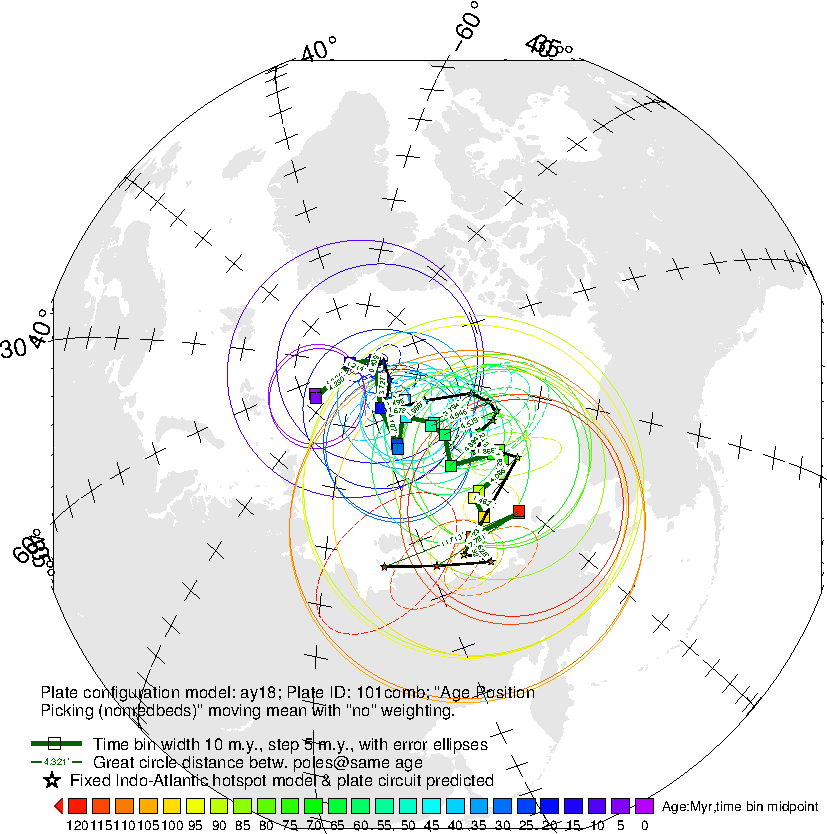
\includegraphics[width=\textwidth]{figures/ay18_101comb_10_5_11_0.pdf}
		\caption{North America: minimum 0.0053 (11, 0)}\label{fig-nac-105110}
	\end{subfigure}
	\begin{subfigure}{.42\textwidth} % width of right subfigure
		\includegraphics[width=\textwidth]{figures/ay18_101comb_10_5_16_3.pdf}
		\caption{North America: maximum 0.0921 (16, 3)}\label{fig-nac-105163}
	\end{subfigure}
	\vspace{.1em}
	\begin{subfigure}{.42\textwidth}
		\includegraphics[width=\textwidth]{figures/ay18_501comb_10_5_19_0.pdf}
		\caption{India: minimum 0.023 (19, 0)}\label{fig-ind-105190}
	\end{subfigure}
	\begin{subfigure}{.42\textwidth}
		\includegraphics[width=\textwidth]{figures/ay18_501comb_10_5_8_3.pdf}
		\caption{India: maximum 0.5137 (8, 3)}\label{fig-ind-10583}
	\end{subfigure}
	\vspace{.1em}
	\begin{subfigure}{.42\textwidth}
		\includegraphics[width=\textwidth]{figures/ay18_801comb_10_5_17_0.pdf}
		\caption{Australia: minimum 0.0037 (17, 0)}\label{fig-au-105170}
	\end{subfigure}
	\begin{subfigure}{.42\textwidth}
		\includegraphics[width=\textwidth]{figures/ay18_801comb_10_5_22_3.pdf}
		\caption{Australia: maximum 0.3954 (22, 3)}\label{fig-au-105223}
	\end{subfigure}
	\caption[Best and worst differences (10 Myr bin, 5 Myr
step)]{Path comparisons with best and worst difference values shown in
Fig.~\ref{fig-dif}. The parenthetical remarks are Picking No and Weighting No.}\label{fig-difbw}
\end{figure*}

\begin{figure*}
	\centering
	\begin{subfigure}{1.01\textwidth}
		\includegraphics[width=\textwidth]{figures/f501d101.pdf}
		\caption{Differences between Fig.~\ref{fig-ind-dif} (India) and
		Fig.~\ref{fig-nac-dif} (North America)}\label{fig-i-n-dif}
	\end{subfigure}
	\vspace{.1em}
	\begin{subfigure}{1.01\textwidth}
		\includegraphics[width=\textwidth]{figures/f801d101.pdf}
		\caption{Differences between Fig.~\ref{fig-au-dif} (Australia) and
		Fig.~\ref{fig-nac-dif} (North America)}\label{fig-a-n-dif}
	\end{subfigure}
	\vspace{.1em}
	\begin{subfigure}{1.01\textwidth}
		\includegraphics[width=\textwidth]{figures/f501d801.pdf}
		\caption{Differences between Fig.~\ref{fig-ind-dif} (India) and
		Fig.~\ref{fig-au-dif} (Australia)}\label{fig-i-a-dif}
	\end{subfigure}
	\caption[Differences of differences of each plate's paleomagnetic
APWPs versus its FHM predicted APWP]{Differences between grids in
Fig.~\ref{fig-dif}. The absolute difference values less than
1.96-standard-deviation interval of the whole 168 values are labeled in green,
more than 1.96-standard-deviation interval labeled in red.}\label{fig-d-dif}
\end{figure*}

\begin{figure*}
	\centering
	\begin{subfigure}{1.01\textwidth}
		\includegraphics[width=\textwidth]{figures/101_120_0APPvsAMP.pdf}
		\caption{AMP: minimum 0.0292 (4/6, 5), maximum 0.0921 (16,
		3), mean 0.04641, median 0.04664; APP: minimum 0.0053 (11, 0), maximum
		0.05686 (5/7, 3), mean 0.02055, median 0.01594}\label{fig-na-difAMPvsAPP}
	\end{subfigure}
	\vspace{.1em}
	\begin{subfigure}{1.01\textwidth}
		\includegraphics[width=\textwidth]{figures/501_120_0APPvsAMP.pdf}
		\caption{AMP: minimum 0.047 (4/6, 3), maximum 0.5137 (8, 3), mean
		0.1684, median 0.1862; APP: minimum 0.023 (19, 0), maximum 0.1359 (3,
		4), mean 0.06786, median 0.0609}\label{fig-in-difAMPvsAPP}
	\end{subfigure}
	\vspace{.1em}
	\begin{subfigure}{1.01\textwidth}
		\includegraphics[width=\textwidth]{figures/801_120_0APPvsAMP.pdf}
		\caption{AMP: minimum 0.0305 (0/20, 3), maximum 0.3954 (22,
		3), mean 0.1264, median 0.0951; APP: minimum 0.0037 (17, 0), maximum
		0.11035 (15, 3), mean 0.04225, median 0.0282}\label{fig-au-difAMPvsAPP}
	\end{subfigure}
	\caption[Differences of each plate's paleomagnetic APWPs versus its FHM
predicted APWP (AMP vs APP)]{Separated results from AMP and APP in
Fig.~\ref{fig-dif}. For each grid block (left: AMP; right: APP), the difference
values less than one-standard-deviation interval of the whole 84 values are
labeled in green, more than one-standard-deviation interval labeled in
red.}\label{fig-difAMPvsAPP}
\end{figure*}


\paragraph{20 Myr Binning and 10 Myr Stepping}

According to the results (Fig.~\ref{fig-dif2010}), we can observe:
%
\begin{enumerate}
  \item the groups of picking-method-no 19 is the best, and 16 the worst, for
        all the three continents.
\end{enumerate}

\begin{figure*}
	\centering
	\begin{subfigure}{1.01\textwidth}
		\includegraphics[width=\textwidth]{figures/101_20_10_120_0.pdf}
		\caption{North America (101 with children): minimum 0.0115 (13, 0), maximum 0.0635 (16, 2), mean 0.0335, median 0.0285}\label{fig-nac-dif2010}
	\end{subfigure}
	\vspace{.1em}
	\begin{subfigure}{1.01\textwidth}
		\includegraphics[width=\textwidth]{figures/501_20_10_120_0.pdf}
		\caption{India (501): minimum 0.0143 (6, 3), maximum 0.1543 (16, 3), mean 0.074, median 0.0755}\label{fig-ind-dif2010}
	\end{subfigure}
	\vspace{.1em}
	\begin{subfigure}{1.01\textwidth}
		\includegraphics[width=\textwidth]{figures/801_20_10_120_0.pdf}
		\caption{Australia (801 with children): minimum 0.0022 (11, 0), maximum 0.3265 (22, 3), mean 0.0686, median 0.0346}\label{fig-au-dif2010}
	\end{subfigure}
	\caption[Differences of each plate's paleomagnetic APWPs versus
its FHM predicted APWP]{Same as Fig.~\ref{fig-dif}. The only difference is here
the paths are in 20 Myr bin and 10 Myr step. The difference values less than
one-standard-deviation interval of the whole 168 values are colored in green,
more than one-standard-deviation interval colored in red. See the numbers
of picked paleopoles in Fig.~\ref{fig-dif}.}\label{fig-dif2010}
\end{figure*}

\begin{figure*}
	\centering
	\begin{subfigure}{.43\textwidth}
		\includegraphics[width=\textwidth]{figures/ay18_101comb_20_10_13_0.pdf}
		\caption{North America: minimum 0.0115 (13, 0)}\label{fig-nac-2010130}
	\end{subfigure}
	\begin{subfigure}{.43\textwidth}
		\includegraphics[width=\textwidth]{figures/ay18_101comb_20_10_16_2.pdf}
		\caption{North America: maximum 0.0635 (16, 2)}\label{fig-nac-2010162}
	\end{subfigure}
	\vspace{.1em}
	\begin{subfigure}{.43\textwidth}
		\includegraphics[width=\textwidth]{figures/ay18_501comb_20_10_6_3.pdf}
		\caption{India: minimum 0.0143 (6, 3)}\label{fig-ind-201063}
	\end{subfigure}
	\begin{subfigure}{.43\textwidth}
		\includegraphics[width=\textwidth]{figures/ay18_501comb_20_10_16_3.pdf}
		\caption{India: maximum 0.1543 (16, 3)}\label{fig-ind-2010163}
	\end{subfigure}
	\vspace{.1em}
	\begin{subfigure}{.43\textwidth}
		\includegraphics[width=\textwidth]{figures/ay18_801comb_20_10_11_0.pdf}
		\caption{Australia: minimum 0.0022 (11, 0)}\label{fig-au-2010110}
	\end{subfigure}
	\begin{subfigure}{.43\textwidth}
		\includegraphics[width=\textwidth]{figures/ay18_801comb_20_10_22_3.pdf}
		\caption{Australia: maximum 0.3265 (22, 3)}\label{fig-au-2010223}
	\end{subfigure}
	\caption[Best and worst differences (20 Myr bin, 10 Myr
step)]{Path comparisons with best and worst difference values shown in
Fig.~\ref{fig-dif2010}. The parenthetical remarks are Picking No and Weighting No.}\label{fig-dif2010bw}
\end{figure*}


\subsubsection{When MHM and Global Plate Tectonic Circuits Predicted APWP as
Reference}

Then, we focus on analysing the results with MHM and global plate circuits
predicted APWP (Fig.~\ref{fig-mhsPred}, Fig.~\ref{fig-mhsPred501},
Fig.~\ref{fig-mhsPred801}) as the reference path.

\begin{figure*}
	\centering
	\begin{subfigure}{1.01\textwidth}
		\includegraphics[width=\textwidth]{figures/101_120_0m.pdf}
		\caption{North America (101 with children): minimum 0.00077 (4, 0), maximum 0.0926 (16, 5), mean 0.0361, median 0.0325}\label{fig-nac-difm}
	\end{subfigure}
	\vspace{1em}
	\begin{subfigure}{1.01\textwidth}
		\includegraphics[width=\textwidth]{figures/501_120_0m.pdf}
		\caption{India (501): minimum 0.0228 (4, 3), maximum 0.5188 (8, 3), mean 0.113, median 0.0746}\label{fig-ind-difm}
	\end{subfigure}
	\vspace{1em}
	\begin{subfigure}{1.01\textwidth}
		\includegraphics[width=\textwidth]{figures/801_120_0m.pdf}
		\caption{Australia (801 with children): minimum 0.0024 (17, 5), maximum 0.3662 (22, 3), mean 0.0744, median 0.0374}\label{fig-au-difm}
	\end{subfigure}
	\caption[Differences of each plate's paleomagnetic APWPs versus
its MHM predicted APWP]{Same as Fig.~\ref{fig-dif} except that the reference
path is predicted from MHM here. See the numbers of picked paleopoles in
Fig.~\ref{fig-dif}.}\label{fig-difm}
\end{figure*}

\begin{figure*}
	\centering
	\begin{subfigure}{.42\textwidth}
		\includegraphics[width=\textwidth]{figures/ay18_101comb_10_5_4_0m.pdf}
		\caption{North America: minimum 0.00077 (4, 0)}\label{fig-nac-10540m}
	\end{subfigure}
	\begin{subfigure}{.42\textwidth}
		\includegraphics[width=\textwidth]{figures/ay18_101comb_10_5_16_5m.pdf}
		\caption{North America: maximum 0.0926 (16, 5)}\label{fig-nac-105165m}
	\end{subfigure}
	\vspace{.1em}
	\begin{subfigure}{.42\textwidth}
		\includegraphics[width=\textwidth]{figures/ay18_501comb_10_5_4_3m.pdf}
		\caption{India: minimum 0.0228 (4, 3)}\label{fig-ind-10543m}
	\end{subfigure}
	\begin{subfigure}{.42\textwidth}
		\includegraphics[width=\textwidth]{figures/ay18_501comb_10_5_8_3m.pdf}
		\caption{India: maximum 0.5188 (8, 3)}\label{fig-ind-10583m}
	\end{subfigure}
	\vspace{.1em}
	\begin{subfigure}{.42\textwidth}
		\includegraphics[width=\textwidth]{figures/ay18_801comb_10_5_17_5m.pdf}
		\caption{Australia: minimum 0.0024 (17, 5)}\label{fig-au-105175m}
	\end{subfigure}
	\begin{subfigure}{.42\textwidth}
		\includegraphics[width=\textwidth]{figures/ay18_801comb_10_5_22_3m.pdf}
		\caption{Australia: maximum 0.3662 (22, 3)}\label{fig-au-105223m}
	\end{subfigure}
	\caption[Best and worst differences (10 Myr bin, 5 Myr
step)]{Path comparisons with best and worst difference values shown in
Fig.~\ref{fig-difm}. The parenthetical remarks are Picking No and Weighting No.}\label{fig-difbwm}
\end{figure*}

\paragraph{10 Myr Binning and 5 Myr Stepping}

According to the results (Fig.~\ref{fig-nac-difm}, Fig.~\ref{fig-ind-difm} and
Fig.~\ref{fig-au-difm}), we can observe:
%
\begin{enumerate}
  \item there is no best picking method, whereas no. 16 is the worst, for all
		the three continents.
\end{enumerate}


\paragraph{20 Myr Binning and 10 Myr Stepping}

According to the results (Fig.~\ref{fig-dif2010m}), we can observe:
%
\begin{enumerate}
  \item there is no best picking method, whereas no. 16 is the worst, for all
		the three continents.
\end{enumerate}

\begin{figure*}
	\centering
	\begin{subfigure}{1.01\textwidth}
		\includegraphics[width=\textwidth]{figures/101_20_10_120_0m.pdf}
		\caption{North America (101 with children): minimum 0.0058 (15, 5), maximum 0.1041 (8, 4), mean 0.0437, median 0.0267}\label{fig-nac-dif2010m}
	\end{subfigure}
	\vspace{1em}
	\begin{subfigure}{1.01\textwidth}
		\includegraphics[width=\textwidth]{figures/501_20_10_120_0m.pdf}
		\caption{India (501): minimum 0.0177 (6, 3), maximum 0.162 (16, 3), mean 0.0759, median 0.0621}\label{fig-ind-dif2010m}
	\end{subfigure}
	\vspace{1em}
	\begin{subfigure}{1.01\textwidth}
		\includegraphics[width=\textwidth]{figures/801_20_10_120_0m.pdf}
		\caption{Australia (801 with children): minimum 0.0047 (23, 4), maximum 0.3158 (26, 3), mean 0.0638, median 0.0307}\label{fig-au-dif2010m}
	\end{subfigure}
	\caption[Differences of each plate's paleomagnetic APWPs versus
its MHM predicted APWP]{Same as Fig.~\ref{fig-dif2010} except that the reference
path is predicted from MHM here. See the numbers of picked paleopoles in
Fig.~\ref{fig-dif}.}\label{fig-dif2010m}
\end{figure*}

\begin{figure*}
	\centering
	\begin{subfigure}{.43\textwidth}
		\includegraphics[width=\textwidth]{figures/ay18_101comb_20_10_15_5m.pdf}
		\caption{North America: minimum 0.0058 (15, 5)}\label{fig-nac-2010155m}
	\end{subfigure}
	\begin{subfigure}{.43\textwidth}
		\includegraphics[width=\textwidth]{figures/ay18_101comb_20_10_8_4m.pdf}
		\caption{North America: maximum 0.1041 (8, 4)}\label{fig-nac-201084m}
	\end{subfigure}
	\vspace{.1em}
	\begin{subfigure}{.43\textwidth}
		\includegraphics[width=\textwidth]{figures/ay18_501comb_20_10_6_3m.pdf}
		\caption{India: minimum 0.0177 (6, 3)}\label{fig-ind-201063m}
	\end{subfigure}
	\begin{subfigure}{.43\textwidth}
		\includegraphics[width=\textwidth]{figures/ay18_501comb_20_10_16_3m.pdf}
		\caption{India: maximum 0.162 (16, 3)}\label{fig-ind-2010163m}
	\end{subfigure}
	\vspace{.1em}
	\begin{subfigure}{.43\textwidth}
		\includegraphics[width=\textwidth]{figures/ay18_801comb_20_10_23_4m.pdf}
		\caption{Australia: minimum 0.0047 (23, 4)}\label{fig-au-2010234m}
	\end{subfigure}
	\begin{subfigure}{.43\textwidth}
		\includegraphics[width=\textwidth]{figures/ay18_801comb_20_10_26_3m.pdf}
		\caption{Australia: maximum 0.3158 (26, 3)}\label{fig-au-2010263m}
	\end{subfigure}
	\caption[Best and worst differences (20 Myr bin, 10 Myr
step)]{Path comparisons with best and worst difference values shown in
Fig.~\ref{fig-dif2010m}. The parenthetical remarks are Picking No and Weighting No.}\label{fig-dif2010bwm}
\end{figure*}


\subsubsection{Summary of Results}

\begin{table*}
\centering
\caption{Performance statistics of all the picking and weighting methods.}
\label{tab-bw}
\resizebox{\textwidth}{!}{%
\begin{tabular}{l|l|l|l|l|l|l|l|l|l|l|l|l|l}
\multicolumn{2}{l|}{\multirow{2}{*}{Grid}} & \multicolumn{2}{l|}{Best No.} &
  \multicolumn{2}{l|}{Worst No.} & \multirow{2}{*}{\parbox{1.8cm}{Proportion of
  APP Better Than AMP}} & \multicolumn{6}{l|}{\multirow{2}{*}{\parbox{5cm}{For
  All 28 Picking Methods, Count of Occurrences of Each Weighting No. Being
  Best}}} & \multirow{2}{*}{\parbox{2.6cm}{Picking 14/15 (Studies After 1983)
  Better Than 16/17 (Older)}} \\ \\ \cline{3-6} \cline{8-13}
\multicolumn{2}{l|}{} & Picking & Weighting & Picking & Weighting &  & 0 & 1 &
  2 & 3 & 4 & 5 &  \\ \hline
\multirow{12}{*}{FHM}
& Fig.~\ref{fig-nac-dif} & \multirow{2}{*}{\parbox{2cm}{1, 4, 5, 7, 11, 13, 15,
  \textbf{19}, \textbf{21}, 25}} & \multirow{2}{*}{\parbox{1cm}{0, 1, 5}} &
  \multirow{2}{*}{\parbox{2cm}{2, 5, 7, 8, 14, \textbf{16}, 17, 18, 22, 26}} &
  \multirow{2}{*}{\parbox{1cm}{0, 1, 2, 3, 4, 5}} & 27/28 & \textbf{15} & 4 & 2 & 3 & 1
  & 4 & Y/Y \\ \\ \cline{2-14}
& Fig.~\ref{fig-ind-dif} & \multirow{2}{*}{\parbox{2cm}{4, 5, 6, 7, 9,
  \textbf{19}, \textbf{21}}} & \multirow{2}{*}{\parbox{1cm}{0, 1, 2, 3, 4, 5}} &
  \multirow{2}{*}{\parbox{2.4cm}{0, 2, 8, 10, 12, \textbf{16}, 18, 20, 24}} &
  \multirow{2}{*}{\parbox{1cm}{0, 1, 2, 3, 4, 5}} & 11/14 & \textbf{17} & 1 & 2 & 7 & 1
  & 0 & Y/Y \\ \\ \cline{2-14}
& Fig.~\ref{fig-au-dif} & \multirow{2}{*}{\parbox{2cm}{1, 11, 13, 17,
  \textbf{19}, \textbf{21}, 25}} & \multirow{2}{*}{\parbox{1cm}{0, 1, 3, 5}} &
  \multirow{2}{*}{\parbox{2.4cm}{2, 6, 14, \textbf{16}, 22, 26}} &
  \multirow{2}{*}{\parbox{1cm}{0, 1, 2, 3, 4, 5}} & 27/28 & \textbf{11} & 4 & 1 & 8 & 3
  & 1 & N/N \\ \\ \cline{2-14}
& Fig.~\ref{fig-nac-dif2010} & \multirow{2}{*}{\parbox{2cm}{1, 4, 5, 7, 11, 13,
  15, \textbf{19}, \textbf{21}, 25}} & \multirow{2}{*}{\parbox{1cm}{0, 1, 3, 5}} &
  \multirow{2}{*}{\parbox{2.4cm}{2, 6, 14, 22, 26}} &
  \multirow{2}{*}{\parbox{1cm}{0, 1, 2, 3, 4, 5}} & 3/4 & \textbf{18} & 6 & 0 & 2 & 4 &
  3 & N(5n1y)/Y \\ \\ \cline{2-14}
& Fig.~\ref{fig-ind-dif2010} & \multirow{2}{*}{\parbox{2cm}{4, 5, 6, 7,
  \textbf{19}}} & \multirow{2}{*}{\parbox{1cm}{0, 1, 2, 3, 4, 5}} &
  \multirow{2}{*}{\parbox{2.4cm}{0, 2, 10, 12, \textbf{16}, 18, 20, 23, 24, 27}} &
  \multirow{2}{*}{\parbox{1cm}{0, 1, 2, 3, 4, 5}} & 59/84 & \textbf{12} & 6 & 0 & 9 & 0
  & 1 & Y/Y(4y2n) \\ \\ \cline{2-14}
& Fig.~\ref{fig-au-dif2010} & \multirow{2}{*}{\parbox{2cm}{1, 11, 13, 17,
\textbf{19}, \textbf{21}, 25}} & \multirow{2}{*}{\parbox{1cm}{0, 1, 3, 4, 5}} &
  \multirow{2}{*}{\parbox{2cm}{2, 14, \textbf{16}, 22, 26}} &
  \multirow{2}{*}{\parbox{1cm}{0, 1, 2, 3, 4, 5}} & 41/42 & 7 & 9 & 0 & \textbf{11} & 1
  & 2 & N/N(4n2y) \\ \\ \hline
\multirow{12}{*}{MHM}
& Fig.~\ref{fig-nac-difm} & \multirow{2}{*}{\parbox{2cm}{1, 4, 5, 7, 11, 13, 15,
  \textbf{21}, 25}} & \multirow{2}{*}{\parbox{1cm}{0, 1, 2, 3, 4, 5}} &
  \multirow{2}{*}{\parbox{2.2cm}{0, 8, 10, 12, 14, \textbf{16}, 17, 18, 20, 22, 24}} &
  \multirow{2}{*}{\parbox{1cm}{0, 1, 2, 3, 4, 5}} & 11/12 & \textbf{14} & 6 & 1 & 1 & 2
  & 4 & Y/Y \\ \\ \cline{2-14}
& Fig.~\ref{fig-ind-difm} & \multirow{2}{*}{\parbox{2cm}{4, 5, 6, 7, \textbf{19}, 22, 26}} &
  \multirow{2}{*}{\parbox{1cm}{0, 1, 2, 3, 4, 5}} &
  \multirow{2}{*}{\parbox{2.4cm}{0, 2, 8, 10, 12, \textbf{16}, 18, 20, 24}} &
  \multirow{2}{*}{\parbox{1cm}{0, 1, 2, 3, 4, 5}} & 11/14 & \textbf{12} & 3 & 0 & 9 & 1
  & 3 & Y/Y \\ \\ \cline{2-14}
& Fig.~\ref{fig-au-difm} & \multirow{2}{*}{\parbox{2cm}{1, 11, 13, 17,
  \textbf{19}, \textbf{21}, 25}} & \multirow{2}{*}{\parbox{1cm}{0, 1, 3, 5}} &
  \multirow{2}{*}{\parbox{2.4cm}{2, 14, \textbf{16}, 22, 26}} &
  \multirow{2}{*}{\parbox{1cm}{0, 1, 2, 3, 4, 5}} & 20/21 & 8 & 5 & 1 & \textbf{9} & 4
  & 1 & N/N \\ \\ \cline{2-14}
& Fig.~\ref{fig-nac-dif2010m} & \multirow{2}{*}{\parbox{2cm}{4, 5, 7, 11,
  15, 22, 26}} & \multirow{2}{*}{\parbox{1cm}{0, 1, 2, 3, 4, 5}} &
  \multirow{2}{*}{\parbox{2.4cm}{0, 8, 10, 12, 14, \textbf{16}, 18, 20, 24}} &
  \multirow{2}{*}{\parbox{1cm}{0, 1, 2, 3, 4, 5}} & 3/4 & \textbf{15} & 6 & 1 & 0 & 1 &
  5 & N(5n1y)/Y \\ \\ \cline{2-14}
& Fig.~\ref{fig-ind-dif2010m} & \multirow{2}{*}{\parbox{2cm}{4, 5, 6, 7,
  \textbf{19}}} & \multirow{2}{*}{\parbox{1cm}{0, 1, 2, 3, 4, 5}} &
  \multirow{2}{*}{\parbox{2.4cm}{0, 2, 10, 12, \textbf{16}, 18, 23, 24, 27}} &
  \multirow{2}{*}{\parbox{1cm}{0, 1, 2, 3, 4, 5}} & 29/42 & \textbf{8} & \textbf{8} & 2 & 5 & 3
  & 2 & Y/N(5n1y) \\ \\ \cline{2-14}
& Fig.~\ref{fig-au-dif2010m} & \multirow{2}{*}{\parbox{2cm}{1, 11, 13, 15, 17,
  \textbf{19}, \textbf{21}, 23, 25, 27}} & \multirow{2}{*}{\parbox{1cm}{0, 1, 2, 3, 4, 5}} &
  \multirow{2}{*}{\parbox{2cm}{2, 14, \textbf{16}, 22, 26}} &
  \multirow{2}{*}{\parbox{1cm}{0, 1, 2, 3, 4, 5}} & 41/42 & \textbf{9} & 5 & 0 & 8 & 5
  & 1 & N/Y(4y2n)
\end{tabular}%
}
\end{table*}

According to all the above results (Fig.~\ref{fig-dif} and
Fig.~\ref{fig-dif2010}), we can observe:
%
\begin{enumerate}
  \item generally the APP methods (adding data to a time window with overlapping
        age selection criterion) produce better similarities than the AMP
        methods (Table.~\ref{tab-bw}).
  \item the self-explanatory topography of bands indicates that the picking
        methods (Table.~\ref{tab-pick}) influence the similarity more than the
        weighting methods (Table.~\ref{tab-weit}) do.
  \item filtering (picking no 2\textendash7, 10, 11, and 14\textendash27) and
        correcting (picking no 8, 9, 12 and 13) has limited effectiveness.
  \item weighting is not always making similarities better. In fact, for quite
        many of the methods, no weighting is the best performer
		(Table.~\ref{tab-bw}).
  \item the picking method no 19 is always the best when the FHM predicted APWP
		is the reference.
  \item the weighting method no 0, 1 and 5 are generally producing better
        similarity than 2, 3 and 4.
  \item North America (101) owns better similarity results than Australia (801)
        and India (501), because its worst and mean composite differences are
		always less than the other two continents'.
  \item for both North America (101) and India (501), more recent studies
        generally give better results than (or results close to) older studies.
		However, this is not true for Australia (801) (Fig.~\ref{fig-au-dif}).
\end{enumerate}

\subsection{Discussions}

The following discussions will be in Q\&A style.

\subsubsection{Question: Why the APP methods generally produce better
similarities than AMP methods do?}

Paleomagnetic (Mean) A95 represents precision (how well constrained calculated
poles are), and (mean) coeval poles' GCD represents accuracy (how close
calculated poles are to the reference path; Fig.~\ref{fig-A95GCD105F} and
Fig.~\ref{fig-A95SGCD105F}). Compared with AMP, APP usually improves both and
generates paths with higher accuracy and also higher precision (generally
increasing N).

\begin{figure}
\captionsetup[subfigure]{singlelinecheck=off,justification=raggedright,aboveskip=-6pt,belowskip=-6pt}
\centering
  \begin{subfigure}[htbp]{.49\textwidth}
	\caption{}\includegraphics[width=\textwidth]{figures/a95gcd_10_5F.pdf}\label{fig-A95GCD105F}
  \end{subfigure}
  \begin{subfigure}[htbp]{.49\textwidth}
	\caption{}\includegraphics[width=\textwidth]{figures/a95Sgcd_10_5F.pdf}\label{fig-A95SGCD105F}
  \end{subfigure}
  \begin{subfigure}[htbp]{.49\textwidth}
	\caption{}\includegraphics[width=\textwidth]{figures/a95mSad10_5F.pdf}\label{fig-A95mSad105F}
  \end{subfigure}
  \begin{subfigure}[htbp]{.49\textwidth}
	\caption{}\includegraphics[width=\textwidth]{figures/a95mSld10_5F.pdf}\label{fig-A95mSld105F}
  \end{subfigure}
\caption[APP spatially better than AMP]{Paleomagnetic APWPs' mean A95 versus
(a) ``mean GCD'', (b) ``mean significant GCD'', (c) ``mean significant
orientation difference'', and (d) ``mean significant length difference'' between
paleomagnetic APWP and its corresponding FHM-and-plate-circuit predicted APWP\@.
Starting points of the arrows are results from AMP, while ending points are from
APP\@. Black color filled arrow heads are the small number of special cases of
AMP derived equal-weight CPDs better than APP (see details in
Fig.~\ref{fig-dif}).}\label{fig-A95mG105F}
\end{figure}

\begin{figure}
\captionsetup[subfigure]{singlelinecheck=off,justification=raggedright,aboveskip=-6pt,belowskip=-6pt}
\centering
  \begin{subfigure}[htbp]{.49\textwidth}
	\caption{}\includegraphics[width=\textwidth]{figures/a95gcdd.pdf}\label{fig-A95GCD105Fd}
  \end{subfigure}
  \begin{subfigure}[htbp]{.49\textwidth}
	\caption{}\includegraphics[width=\textwidth]{figures/a95Sgcd_10_5Fd.pdf}\label{fig-A95SGCD105Fd}
  \end{subfigure}
  \begin{subfigure}[htbp]{.49\textwidth}
	\caption{}\includegraphics[width=\textwidth]{figures/a95mSad10_5Fd.pdf}\label{fig-A95mSad105Fd}
  \end{subfigure}
  \begin{subfigure}[htbp]{.49\textwidth}
	\caption{}\includegraphics[width=\textwidth]{figures/a95mSld10_5Fd.pdf}\label{fig-A95mSld105Fd}
  \end{subfigure}
\caption[APP spatially better than AMP]{Differences of APP and AMP coordinates
shown in Fig.~\ref{fig-A95mG105F}. Crosses locates the small minority cases of
AMP derived equal-weight CPDs better than APP (see details in
Fig.~\ref{fig-dif}).}\label{fig-A95mG105Fd}
\end{figure}

The fact that APP increases the number of paleopoles (N) in each sliding window
would potentially average out some ``bad'' (i.e.\ inaccurate) poles and improves
the fit between the paleomagnetic APWPs and the model-predicted APWPs. The
general effects that APP brings include the decreases in paleomagnetic A95s,
or/and distances between compared coeval poles of paleomagnetic APWP and
reference APWP (Fig.~\ref{fig-A95mG105F} and Fig.~\ref{fig-A95mG105Fd}).
However, if the added paleopoles were all or mostly ``bad'', the improvement of
fit would not occur. So the improvement of fit is not only because of the
increase in N, but also because the majority of the additional poles are
``good''. AMP only regards the time uncertainty of each pole as one mid-point.
Then this mid-point is treated as the most likely age of that mean pole. This is
actually incorrect. The age uncertainty of paleopole is not obtained from a
probability density function derived from an observed frequency distribution. As
defined, the time uncertainty's lower (older) limit is a stratigraphic age, and
its upper (younger) limit could be also a stratigraphic age or be constrained by
a tectonic event using the field tests (e.g.\ fold/tilt test and conglomerate
test). So the true age of the pole could be any one that is not older than the
lower limit and also not younger than the upper limit. In other words, the
mid-point could be the true age of the pole, but it is not known as the most
likely age of that pole. If the mid-point is the most likely age of a pole, AMP
should generate a path that is closer to the reference. However, mostly APP
generates better similarities (See the high proportions of APP better than AMP
in Table.~\ref{tab-bw}). Most reasonably, the mid-point should be regarded as
one possibility of all uniformly (not necessarily normally bell shaped, or U
shaped, or left or right skewed) distributed ages between the two time limits.

So APP remains the effect of a paleopole borne on the mean poles during all the
period of its age uncertainty, and use the increased number of paleopoles (N)
to average out the negative effect of those ``bad'' poles, including the
paleopoles that should not be included at that age for mean pole.

\subsubsection{Question: Why the AMP methods sometimes unexceptionally produce
better similarities than APP methods do?}

Because of small number of paleopoles (not necessarily ``bad'') involved in
each sliding window, the produced mean poles by AMP should be relatively far
from its contemporary model-predicted pole. In other words, AMP intends to give
fairly small change in accuracy. This also could potentially bring more
distinguishable $d_s$ for AMP\@ if the corresponding A95 is not large enough.
For example, for Fig.~\ref{fig-nac-dif}, there are only three special (of 84 APP
vs. AMP comparisons) cases picking/weighting 4/3, 4/5, 6/3 better than 5/3, 5/5,
7/3 respectively. Compared with the picking/weighting 4/3 APWP, although most of
the mean paleopoles are closer to the FHM predicted APWP and also the number of
the significant pole pairs is one less for the APP derived path (i.e. 5/3), the
A95s are smaller and most importantly there are one more significant $d_a$
orientation-change pair and two more significant $d_l$ segment pair
(Table.~\ref{tab-w3p4vs5}). If we observe carefully, it is because of the much
smaller 15 Ma A95 for 5/3. The similar phenomenon occurs to the case of 6/3 vs
7/3, a relatively much smaller paleomagnetic A95 causes more distinguishable
$d_a$ and $d_l$ for the APP results, and they offset the improvement of spatial
similarity $d_s$ APP brings.

For 4/5 vs 5/5, all $d_a$ and $d_l$ are indistinguishable. Compared with the
results from AMP, although the coeval pole GCDs are all decreased for APP, this
spatial improvement is not able to offset the negative effects of also
generally decreased paleomagnetic A95s, which potentially brings more
statistically distinguishable coeval poles (e.g.\ the 15 Ma and 30 Ma poles for
picking 5 and weighting 5; Table.~\ref{tab-w5p4vs5}). This further causes
greater distinguishable mean $d_s$ from the APP methods. The similar phenomenon
occurs to Fig.~\ref{fig-ind-dif} picking 4 vs 5 with all the six types of
weightings, Fig.~\ref{fig-au-dif} picking/weighting 4/2\textendash3 vs
5/2\textendash3, 4/5 vs 5/5.

In addition, compared with AMP, APP potentially could generate more mean poles,
because sometimes for some sliding window there is no paleopole involved at all
for AMP\@ while there is(are) paleopole(s) involved for APP\@. For APP, the
mean poles at all ages should be composed of more paleopoles than it is for
AMP, which should generally decrease both coeval pole distance and paleomagnetic
A95. However, sometimes a rare case (e.g.\ the 0 Ma comparison shown in
Table.~\ref{tab-501w0p22vs23}) happens. It is sometimes that an additional
very ``bad'' paleopole gets included by APP and this increases both coeval pole
distance and paleomagnetic A95 even though N increases. Such cases include
Fig.~\ref{fig-ind-dif} picking 22 vs 23 (actually exactly the same as picking 26
vs 27) with all the six types of weightings.

So generally as we discussed in the last section APP decreases the distances
between paleomagnetic APWPs and the hotspot and sea-floor spreading model
predicted APWP, and also the uncertainties of paleomagnetic APWPs. However, as
we described in this section, special cases like decreased A95 potentially
intends to make coeval poles differentiated if the coeval poles' distance is
not decreased effectively or even increased, or very ``bad'' paleopoles got
involved in some sliding windows, occurs. In summary, when the negative effect
from these types of rare cases is beyond the positive effect the generally
improved mean poles contribute, the composite difference score would increase.
However, this phenomenon seldom occur (Table.~\ref{tab-bw}).

\begin{table*}
\centering
\caption{One example of the Type 1 rare cases where AMP gives better similarity
  result than APP does from North America (101). Only statistically significant
  values are listed here.}
\label{tab-w3p4vs5}
\resizebox{\textwidth}{!}{%
\begin{tabular}{|c|l|l|l|l|l|l|l|l|l}
\hline
\multicolumn{2}{|c|}{\multirow{2}{*}{FHM predicted}} & \multicolumn{3}{c|}{picking 4 + weighting 3} & \multicolumn{5}{c|}{picking 5 + weighting 3} \\ \cline{3-10} 
\multicolumn{2}{|c|}{} & \multicolumn{3}{c|}{ds} & \multicolumn{3}{c|}{ds} & \multicolumn{2}{c|}{da} \\ \hline
Age (Ma) & \multicolumn{1}{c|}{A95 (\degree)} & \multicolumn{1}{c|}{Age (Ma)} & \multicolumn{1}{c|}{Pmag A95 (\degree)} & \multicolumn{1}{c|}{Dist (\degree)} & \multicolumn{1}{c|}{Age (Ma)} & \multicolumn{1}{c|}{Pmag A95 (\degree)} & \multicolumn{1}{c|}{Dist (\degree)} & \multicolumn{1}{c|}{Age (Ma)} & \multicolumn{1}{c|}{Diff (\degree)} \\ \hline
0 & 0 & 0 & 8.3 & \textbf{4.29} & 0 & 7.6 & \textbf{3.885} & \textit{\textbf{10-15-20}} & \multicolumn{1}{l|}{\textbf{126.59}} \\ \hline
5 & 1.56039/0.87367 & 5 & 7 & \textbf{4.853} & 5 & 6.8 & \textbf{4.3453} & \multicolumn{2}{l|}{} \\ \hline
10 & 2.89214/1.58743 & 10 & 12 & \textbf{9.91} & 10 & 8.6 & \textbf{5.79} & \multicolumn{2}{c|}{dl} \\ \hline
15 & 2.575/1.63303 & 15 & 58/49 & \textbf{6.72} & 15 & 2.0857 & \textbf{11.8} & Age (Ma) & \multicolumn{1}{l|}{Diff (\degree)} \\ \hline
20 & 3.16077/2.20094 & \textit{\textbf{20}} & 12.43 & \textbf{8.58} & \multicolumn{3}{l|}{} & \textit{\textbf{10-15}} & \multicolumn{1}{l|}{\textbf{13.52}} \\ \hline
25 & 4.96061/2.2183 & 25 & 6.76 & \textbf{6.96} & 25 & 6.3358 & \textbf{6.873} & \textit{\textbf{15-20}} & \multicolumn{1}{l|}{\textbf{14.68}} \\ \hline
30 & 3.39692/2.57114 & 30 & 6.68 & \textbf{6.46} & 30 & 6.68 & \textbf{6.4583} & \multicolumn{2}{l|}{\multirow{3}{*}{}} \\ \cline{1-8}
115 & 9.27023/5.16012 & 115 & 8.6 & \textbf{12.2535} & 115 & 8.5 & \textbf{11.7} & \multicolumn{2}{l|}{} \\ \cline{1-8}
120 & 14.6882/8.12086 & 120 & 7.76 & \textbf{15.5744} & 120 & 7.728 & \textbf{15.258} & \multicolumn{2}{l|}{} \\ \cline{1-8}
\end{tabular}%
}
\end{table*}

\begin{table*}
\caption{One example of the Type 2 rare cases where AMP gives better similarity
  result than APP does from North America (101). Only statistically significant
  values are listed here. Note that the number of the ages of the significant
  differentiated mean poles are the same for both paleomagnetic APWPs in this
  type of situation.}
\label{tab-w5p4vs5}
\begin{tabular}{|c|l|l|l|l|l|}
\hline
\multirow{3}{*}{\begin{tabular}[c]{@{}c@{}}Age \\ \\ (Ma)\end{tabular}} & \multicolumn{1}{c|}{\multirow{2}{*}{FHM predicted}} & \multicolumn{4}{c|}{ds} \\ \cline{3-6} 
 & \multicolumn{1}{c|}{} & \multicolumn{2}{l|}{picking 4 + weighting 5} &
  \multicolumn{2}{l|}{picking 5 + weighting 5} \\ \cline{2-6} 
 & \multicolumn{1}{c|}{A95 (\degree)} & \multicolumn{1}{c|}{Pmag A95 (\degree)} & \multicolumn{1}{c|}{Dist (\degree)} & \multicolumn{1}{c|}{Pmag A95 (\degree)} & \multicolumn{1}{c|}{Dist (\degree)} \\ \hline
0 & 0 & 8.3526 & \textbf{3.79} & 7.6664 & \textbf{3.391} \\ \hline
5 & 1.56039/0.87367 & 7.5215 & \textbf{4.17} & 7.29 & \textbf{3.74} \\ \hline
10 & 2.89214/1.58743 & 21.351 & \textbf{4.76} & 14.598 & \textbf{2.87} \\ \hline
15 & 2.575/1.63303 & \multicolumn{2}{l|}{\multirow{2}{*}{}} & 10.153 & \textbf{10.71} \\ \cline{1-2} \cline{5-6} 
30 & 3.39692/2.57114 & \multicolumn{2}{l|}{} & 6.9664 & \textbf{5.7245} \\ \hline
115 & 9.27023/5.16012 & 9.635 & \textbf{11.935} & 9.452 & \textbf{11.276} \\ \hline
120 & 14.6882/8.12086 & 8.0223 & \textbf{15.8183} & 7.943 & \textbf{15.511} \\ \hline
\end{tabular}%
\end{table*}

\begin{table*}
\centering
\caption{One example of the Type 3 rare cases where AMP gives better similarity
  result than APP does from India (501). Only statistically significant values
  are listed here. Note that for the bold-number ages, there is no mean poles
  at all for the ``picking 22 (AMP) + weighting 0'' case.}
\label{tab-501w0p22vs23}
\begin{tabular}{|l|l|l|l|l|l|l|l|l|l}
\hline
\multicolumn{2}{|c|}{\multirow{2}{*}{FHM predicted}} & \multicolumn{3}{c|}{picking 22 + weighting 0} & \multicolumn{5}{c|}{picking 23 + weighting 0} \\ \cline{3-10} 
\multicolumn{2}{|c|}{} & \multicolumn{3}{c|}{ds} & \multicolumn{3}{c|}{ds} & \multicolumn{2}{c|}{dl} \\ \hline
\multicolumn{1}{|c|}{Age (Ma)} & \multicolumn{1}{c|}{A95 (\degree)} & \multicolumn{1}{c|}{Pmag A95 (\degree)} & Dist (\degree) & N & \multicolumn{1}{c|}{Pmag A95 (\degree)} & Dist (\degree) & N & Age (Ma) & \multicolumn{1}{l|}{Diff (\degree)} \\ \hline
0 & 0 & \textbf{6.85} & \textbf{12.973} & \textit{\textbf{2}} & \textbf{23.6214} & \textbf{17.698} & \textit{\textbf{3}} & \textbf{80-85} & \multicolumn{1}{l|}{6.286} \\ \hline
5 & 1.415/0.965 & 23.6214 & 15.941 & 3 & 23.6214 & 15.941 & 3 & \textbf{110-115} & \multicolumn{1}{l|}{16.684} \\ \hline
10 & 2.2425/1.34645 & 5.4/3.1 & 29.897 & 1 & 5.4/3.1 & 29.897 & 1 & \multicolumn{2}{l|}{\multirow{12}{*}{}} \\ \cline{1-8}
\textbf{15} & 2.2694/1.62543 & \multicolumn{3}{l|}{\textbf{}} & 5.4/3.1 & 28.28 & 1 & \multicolumn{2}{l|}{} \\ \cline{1-8}
70 & 8.53016/4.97567 & 4.0164 & 4.864 & 16 & 3.246 & 4.436 & 20 & \multicolumn{2}{l|}{} \\ \cline{1-8}
\textbf{75} & 5.3554/3.1595 & \multicolumn{3}{l|}{\multirow{2}{*}{\textbf{}}} & 5 & 4.477 & 1 & \multicolumn{2}{l|}{} \\ \cline{1-2} \cline{6-8}
\textbf{80} & 8.41657/5.00588 & \multicolumn{3}{l|}{} & 5 & 3.358 & 1 & \multicolumn{2}{l|}{} \\ \cline{1-8}
85 & 5.01489/2.49492 & 5 & 7.632 & 1 & 5 & 7.632 & 1 & \multicolumn{2}{l|}{} \\ \cline{1-8}
\textbf{90} & 7.77997/2.86845 & \multicolumn{3}{l|}{\multirow{5}{*}{}} & 5 & 10.884 & 1 & \multicolumn{2}{l|}{} \\ \cline{1-2} \cline{6-8}
\textbf{95} & 4.46779/3.24941 & \multicolumn{3}{l|}{} & 5 & 11.099 & 1 & \multicolumn{2}{l|}{} \\ \cline{1-2} \cline{6-8}
\textbf{100} & 5.6124/5.19639 & \multicolumn{3}{l|}{} & 5 & 11.4155 & 1 & \multicolumn{2}{l|}{} \\ \cline{1-2} \cline{6-8}
\textbf{105} & 4.64657/3.49277 & \multicolumn{3}{l|}{} & 5 & 14.908 & 1 & \multicolumn{2}{l|}{} \\ \cline{1-2} \cline{6-8}
\textbf{110} & 9.11039/4.98436 & \multicolumn{3}{l|}{} & 6.8/4.9 & 13.962 & 1 & \multicolumn{2}{l|}{} \\ \cline{1-8}
115 & 9.27023/5.16012 & 10.73 & 10.508 & 5 & 10.73 & 10.508 & 5 & \multicolumn{2}{l|}{} \\ \cline{1-8}
\end{tabular}
\end{table*}

Other Type 1 (e.g. Table.~\ref{tab-w3p4vs5}) cases: Fig.~\ref{fig-nac-dif2010}
picking/weighting 22/3 vs 23/3. Fig.~\ref{fig-nac-difm} 6/3 vs 7/3.

Other Type 2 (e.g. Table.~\ref{tab-w5p4vs5}) cases: Fig.~\ref{fig-nac-dif2010}
picking/weighting 2/0\textendash5 vs 3/0\textendash5, 4/0\textendash2 vs
5/0\textendash2, 4/4 vs 5/4, 6/5 vs 7/5, 6/2\textendash3 vs 7/2\textendash3,
22/4\textendash5 vs 23/4\textendash5, 22/1 vs 23/1, 26/4 vs 27/4, 26/2 vs 27/2.
Fig.~\ref{fig-ind-dif2010} 14/3 vs 15/3. Fig.~\ref{fig-au-dif2010} 4/2 vs 5/2.
Fig.~\ref{fig-nac-difm} 4/0\textendash1 vs 5/0\textendash1.
Fig.~\ref{fig-ind-difm} 4/0\textendash4 vs 5/0\textendash4, 22/0\textendash1 vs
23/0\textendash1, 22/3\textendash4 vs 23/3\textendash4, Fig.~\ref{fig-au-difm}
4/3 vs 5/3, 4/0 vs 5/0, 8/5 vs 9/5, 8/3 vs 9/3. Fig.~\ref{fig-ind-dif2010m}
14/2\textendash3 vs 15/2\textendash3. Fig.~\ref{fig-au-dif2010m} 4/4 vs 5/4.

Combination of both Type 1 and 2 cases: Fig.~\ref{fig-nac-dif2010}
picking/weighting 26/0\textendash1 vs 27/0\textendash1. Fig.~\ref{fig-nac-difm}
4/3 vs 5/3. Fig.~\ref{fig-ind-difm} 22/2 vs 23/2, 22/5 vs 23/5, 26/0\textendash5
vs 27/0\textendash5.

Other Type 3 (e.g. Table.~\ref{tab-501w0p22vs23}) cases: Fig.~\ref{fig-ind-dif2010}
picking/weighting 6/0\textendash5 vs 7/0\textendash5, 22/0\textendash5 vs
23/0\textendash5, 26/0\textendash5 vs 27/0\textendash5. Fig.~\ref{fig-nac-difm}
4/2\textendash5 vs 5/2\textendash5. Fig.~\ref{fig-nac-dif2010m} 2/0\textendash5
vs 3/0\textendash5, 4/2 vs 5/2, 4/4 vs 5/4, 6/2 vs 7/2, 22/0\textendash5 vs
23/0\textendash5, 26/0\textendash5 vs 27/0\textendash5.
Fig.~\ref{fig-ind-dif2010m} 6/0\textendash5 vs 7/0\textendash5, 22/0\textendash5
vs 23/0\textendash5, 26/0\textendash5 vs 27/0\textendash5.


\subsubsection{Question: Why weighting is not affecting?}

Generally, weighting does not affect the similarities dramatically, because the
six results from the six weighting methods are mostly very close. There are a
few special cases that one of them dramatically changes similarity (e.g.\ for
picking method (Pk) 5 and weighting method (Wt) 3, etc.;
Fig.~\ref{fig-nac-dif}). As follows, those normal cases with close results are
discussed first. Those rare cases are examined later.

For Pk 0 in the North America (101) example (Fig.~\ref{fig-nac-dif}), the reason
of why Wt 1\textendash4 do not produce better similarity scores than Wt 0 (i.e.\
no weighting) does is examined here. Take the comparison between Wt 0 and Wt 1
(Table.~\ref{tab-101p0w0vs1}) as an example, although APP indeed decreases the
values of most distances from the reference and most A95s, APP also brings one
more significant differentiated segment-length difference (80\textendash85 Ma
coeval segments; Fig.~\ref{fig-101_8085}) because of the slightly larger A95 and
shorter coeval pole GCD for 80 Ma Pk 0 Wt 1. Although they are distinguishable,
the overlapping of their distributions is quite small
(Fig.~\ref{fig-nac105_00vs01dl}). Wt 2 and 4 cause one more pair of
distinguishable mean poles ($d_s$) than other weighting methods. However,
compared with Wt 0, Wt 5 (i.e.\ combination of $\alpha$95 and age error position
to bin) does affect and bring the best similarity, because Wt 5 decreases the
GCDs of the 20, 80 and especially 100 Ma distinguishable pole pairs (by more
than 2 degrees; Table.~\ref{tab-101p0w0vs1}).

\begin{figure}
\captionsetup[subfigure]{singlelinecheck=off,justification=raggedright,aboveskip=-6pt,belowskip=-6pt}
	\centering
	\begin{subfigure}{.49\textwidth}
		\caption{}\label{fig-nac105_00vs01}
		\includegraphics[width=\textwidth]{figures/ay18_101comb_10_5_0_0vs0_1.pdf}
	\end{subfigure}
	\vspace{1em}
	\begin{subfigure}{.49\textwidth}
		\caption{}\label{fig-nac105_00vs01dl}
		\includegraphics[width=\textwidth]{figures/ay18_101comb10_5_0_0vs1_80_85dl.pdf}
	\end{subfigure}
	\caption[101 10 5 0 0 vs 0 1 80\textendash85 Ma dl]{Significance testing on
the 80\textendash85 segment length difference between North American
paleomagnetic APWPs derived from picking 0 and weightings 0 and 1 and the FHM
predicted APWP (Fig.~\ref{fig-mhsPred}; Table.~\ref{tab-101p0w0vs1}). (a) The
thin segment through stars is from FHM predicted path, and the bold solid and
dashed are from paleomagnetic paths. (b) The results from Wt 1 are
differentiated (Fig.~\ref{fig-na-dlw0} and
Fig.~\ref{fig-na-dlw1}).}\label{fig-101_8085}
\end{figure}

For Fig.~\ref{fig-nac-dif} Pk 1, Wt 0 generates the best similarity. Wt
2\textendash5 cause at least 3 more pairs of distinguishable mean poles ($d_s$)
than other weighting methods. Wt 1 increases the GCDs of all the distinguishable
pole pairs (0, 5 and 120 Ma).

For Fig.~\ref{fig-nac-dif} Pk 2, Wt 0 generates the best similarity. Wt
1\textendash5 cause at least 1 more pair of distinguishable mean poles ($d_s$)
than Wt 0 (60 Ma). Wt 4 also increases another pair of distinguishable mean 
poles ($d_s$) (80 Ma).

\begin{table*}
\centering
\caption{My caption}
\label{tab-101p0w0vs1}
\begin{tabular}{|l|l|l|l|l|l|l|l|l|l|}
\hline
\multicolumn{2}{|c|}{\multirow{2}{*}{FHM predicted for 101}} & \multicolumn{2}{c|}{Pk 0 + Wt 0} & \multicolumn{4}{c|}{Pk 0 + Wt 1} & \multicolumn{2}{c|}{Pk 0 + Wt 5} \\ \cline{3-10} 
\multicolumn{2}{|c|}{} & \multicolumn{2}{c|}{ds} & \multicolumn{2}{c|}{ds} & \multicolumn{2}{c|}{dl} & \multicolumn{2}{c|}{ds} \\ \hline
\multicolumn{1}{|c|}{Age (Ma)} & \multicolumn{1}{c|}{A95 (\degree)} & \multicolumn{1}{c|}{Pmag A95 (\degree)} & Dist (\degree) & \multicolumn{1}{c|}{Pmag A95 (\degree)} & Dist (\degree) & Age (Ma) & Diff (\degree) & Pmag A95 (\degree) & Dist (\degree) \\ \hline
0 & 0 & 4.27286602 & 5.01 & 3.950661 & \textbf{5.05647} & \textbf{80-85} & \textbf{11.103} & 4.143 & 5.356 \\ \hline
5 & 1.56039/0.87367 & 4.22350537 & 5.146 & 3.936601 & 5.1286 & \multicolumn{2}{l|}{\multirow{12}{*}{\textbf{}}} & 4.0534 & 5.407 \\ \cline{1-6} \cline{9-10} 
10 & 2.89214/1.58743 & 20.9920176 & 3.076 & 19.826829 & \textbf{3.22624} & \multicolumn{2}{l|}{} & 19.868 & 3.36 \\ \cline{1-6} \cline{9-10} 
15 & 2.575/1.63303 & 13.8698147 & 10.3 & 13.827757 & \textbf{10.34} & \multicolumn{2}{l|}{} & 13.85 & 10.2753 \\ \cline{1-6} \cline{9-10} 
20 & 3.16077/2.20094 & 8.36501201 & 7.2162 & \textbf{8.463096} & 6.9973 & \multicolumn{2}{l|}{} & 8.413 & \textbf{6.7906} \\ \cline{1-6} \cline{9-10} 
50 & 7.15565/3.22656 & 4.3991229 & 6.22 & \textbf{4.651517} & \textbf{6.273} & \multicolumn{2}{l|}{} & 4.3326 & 6.3563 \\ \cline{1-6} \cline{9-10} 
55 & 7.17564/4.28065 & 5.6991191 & 8.647 & 5.670719 & \textbf{9.6724} & \multicolumn{2}{l|}{} & 5.52 & 8.53 \\ \cline{1-6} \cline{9-10} 
60 & 9.71876/6.35204 & 7.71537555 & 9.498 & 6.889233 & 8.607 & \multicolumn{2}{l|}{} & 7.77 & 9.8237 \\ \cline{1-6} \cline{9-10} 
80 & 8.76515/5.14459 & 6.29356332 & 9.26 & \textbf{6.452368} & 8.098 & \multicolumn{2}{l|}{} & 6.033 & \textbf{8.369} \\ \cline{1-6} \cline{9-10} 
85 & 5.54221/2.65419 & 8.7/6.7 & 18.995 & 8.7/6.7 & 18.995 & \multicolumn{2}{l|}{} & 8.7/6.7 & 18.995 \\ \cline{1-6} \cline{9-10} 
100 & 5.79659/5.36693 & 10.2720657 & 10.75658 & 9.286878 & 9.035 & \multicolumn{2}{l|}{} & 9.045 & \textbf{8.68} \\ \cline{1-6} \cline{9-10} 
115 & 9.27023/5.16012 & 19.767437 & 9.074 & 18.483547 & \textbf{10.054} & \multicolumn{2}{l|}{} & 19.652 & 9.3547 \\ \cline{1-6} \cline{9-10} 
120 & 14.6882/8.12086 & 3.56957955 & 17.3331 & 3.060561 & 17.062 & \multicolumn{2}{l|}{} & 3.606 & 17.47 \\ \cline{1-6} \cline{9-10} 
\end{tabular}
\end{table*}

As the above examples shown, although no weighting is often better than
weighting, the results are actually rather close to each other and also APP
still improves precision and accuracy of most poles for the cases with larger
difference scores, although APP brings extra significant differences in shape
metrics which is also the main cause of their larger difference scores
(Table.~\ref{tab-101p0w0vs1}). However, APP does not always improves precision
or accuracy, for example, for the Pt 5 (mainly or only igneous derived) and Wt 3
(according to $\alpha$95) results (Table.~\ref{tab-101p5}). For Pt 5, the result
with no weighting is still the best, and the results from Wt 0\textendash2, 4, 5
are close and APP generally improves precision and accuracy, just like the above
mentioned general cases. Only for Wt 3, APP worsens precision and improves
accuracy of most poles at the same time. This makes the difference score
dramatically larger than others. In addition, Wt 3 brings more significant
differences in shape metrics, which causes the difference score even larger
(Table.~\ref{tab-101p5}). That Wt 3 sometimes gives dramatical worse similarity
could be related to the way we do the weighting according to the size of
$\alpha$95, i.e.\, the smaller the $\alpha$95 is, the larger the assigned
weight is (see more details about Weighting No. 3 in the Weighting paragraph).
However, small size of $\alpha$95 (high accuracy) could be becausei of those
sampled directions not covering enough long period (thought to be at least about
$10^4$ years) to ``average out'' secular variation for giving a paleopole. That
is to say, the smallest $\alpha$95s could get the greatest weights that they
should not deserve.

\begin{table*}
\centering
\caption{Highest and lowest values for the same variable are highlighted in red
  and green respectively.}
\label{tab-101p5}
\resizebox{\textwidth}{!}{%
\begin{tabular}{|l|l|llllllllllllll}
\hline
\multicolumn{2}{|c|}{} & \multicolumn{2}{c|}{Pk 5 + Wt 0} & \multicolumn{2}{c|}{Pk 5 + Wt 1} & \multicolumn{2}{c|}{Pk 5 + Wt 2} & \multicolumn{4}{c|}{Pk 5 + Wt 3} & \multicolumn{2}{c|}{Pk 5 + Wt 4} & \multicolumn{2}{c|}{Pk 0 + Wt 5} \\ \cline{3-16} 
\multicolumn{2}{|c|}{\multirow{-2}{*}{FHM predicted for 101}} & \multicolumn{2}{c|}{ds} & \multicolumn{2}{c|}{ds} & \multicolumn{2}{c|}{ds} & \multicolumn{2}{c|}{ds} & \multicolumn{2}{c|}{da} & \multicolumn{2}{c|}{ds} & \multicolumn{2}{c|}{ds} \\ \hline
\multicolumn{1}{|c|}{Age (Ma)} & \multicolumn{1}{c|}{A95 (\degree)} & \multicolumn{1}{c|}{Pmag A95 (\degree)} & \multicolumn{1}{l|}{Dist (\degree)} & \multicolumn{1}{l|}{Pmag A95 (\degree)} & \multicolumn{1}{l|}{Dist (\degree)} & \multicolumn{1}{l|}{Pmag A95 (\degree)} & \multicolumn{1}{l|}{Dist (\degree)} & \multicolumn{1}{c|}{Pmag A95 (\degree)} & \multicolumn{1}{l|}{Dist (\degree)} & \multicolumn{1}{l|}{Age (Ma)} & \multicolumn{1}{l|}{Diff (\degree)} & \multicolumn{1}{c|}{Pmag A95 (\degree)} & \multicolumn{1}{c|}{Dist (\degree)} & \multicolumn{1}{l|}{Pmag A95 (\degree)} & \multicolumn{1}{l|}{Dist (\degree)} \\ \hline
0 & 0 & \multicolumn{1}{l|}{7.458} & \multicolumn{1}{l|}{2.058} & \multicolumn{1}{l|}{7.4575} & \multicolumn{1}{l|}{2.387} & \multicolumn{1}{l|}{8.027} & \multicolumn{1}{l|}{3.539} & \multicolumn{1}{l|}{7.598} & \multicolumn{1}{l|}{{\color[HTML]{FE0000} \textbf{3.885}}} & \multicolumn{1}{l|}{10-15-20} & \multicolumn{1}{l|}{{\color[HTML]{FE0000} \textbf{126.5907}}} & \multicolumn{1}{l|}{7.7351} & \multicolumn{1}{l|}{3.624} & \multicolumn{1}{l|}{7.67} & \multicolumn{1}{l|}{3.3909} \\ \hline
5 & 1.56039/0.87367 & \multicolumn{1}{l|}{7.3814} & \multicolumn{1}{l|}{2.624} & \multicolumn{1}{l|}{7.3814} & \multicolumn{1}{l|}{2.995} & \multicolumn{1}{l|}{7.887} & \multicolumn{1}{l|}{3.876} & \multicolumn{1}{l|}{{\color[HTML]{32CB00} \textbf{6.8}}} & \multicolumn{1}{l|}{{\color[HTML]{FE0000} \textbf{4.3453}}} & \multicolumn{2}{l}{\textbf{}} & \multicolumn{1}{l|}{7.515} & \multicolumn{1}{l|}{3.9475} & \multicolumn{1}{l|}{7.29} & \multicolumn{1}{l|}{3.74} \\ \hline
10 & 2.89214/1.58743 & \multicolumn{4}{l|}{} & \multicolumn{1}{l|}{15.208} & \multicolumn{1}{l|}{3.402} & \multicolumn{1}{l|}{{\color[HTML]{32CB00} \textbf{8.602}}} & \multicolumn{1}{l|}{{\color[HTML]{FE0000} \textbf{5.79}}} & \multicolumn{2}{c|}{dl} & \multicolumn{1}{l|}{16.783} & \multicolumn{1}{l|}{4.2726} & \multicolumn{1}{l|}{14.598} & \multicolumn{1}{l|}{2.87} \\ \hline
15 & 2.575/1.63303 & \multicolumn{1}{l|}{12.421} & \multicolumn{1}{l|}{9.2} & \multicolumn{1}{l|}{12.4213} & \multicolumn{1}{l|}{9.077} & \multicolumn{1}{l|}{12.384} & \multicolumn{1}{l|}{9.4} & \multicolumn{1}{l|}{{\color[HTML]{32CB00} \textbf{2.0857}}} & \multicolumn{1}{l|}{{\color[HTML]{FE0000} \textbf{11.805}}} & \multicolumn{1}{l|}{Age (Ma)} & \multicolumn{1}{l|}{Diff (\degree)} & \multicolumn{1}{l|}{12.3843} & \multicolumn{1}{l|}{9.4} & \multicolumn{1}{l|}{10.153} & \multicolumn{1}{l|}{10.71} \\ \hline
20 & 3.16077/2.20094 & \multicolumn{8}{l}{} & \multicolumn{1}{l|}{10-15} & \multicolumn{1}{l|}{{\color[HTML]{FE0000} \textbf{13.52}}} & \multicolumn{2}{l}{} & \multicolumn{2}{l}{} \\ \cline{1-2} \cline{5-6} \cline{9-14}
25 & 4.96061/2.2183 & \multicolumn{2}{l}{} & \multicolumn{1}{l|}{6.463} & \multicolumn{1}{l|}{6.2097} & \multicolumn{2}{l}{} & \multicolumn{1}{l|}{{\color[HTML]{32CB00} \textbf{6.336}}} & \multicolumn{1}{l|}{{\color[HTML]{FE0000} \textbf{6.873}}} & \multicolumn{1}{l|}{15-20} & \multicolumn{1}{l|}{{\color[HTML]{FE0000} \textbf{14.68}}} & \multicolumn{1}{l|}{6.435} & \multicolumn{1}{l|}{6.68} & \multicolumn{2}{l}{\multirow{-2}{*}{}} \\ \cline{1-2} \cline{5-6} \cline{9-16} 
30 & 3.39692/2.57114 & \multicolumn{4}{l}{} & \multicolumn{2}{l}{} & \multicolumn{1}{l|}{{\color[HTML]{32CB00} \textbf{6.678}}} & \multicolumn{1}{l|}{{\color[HTML]{FE0000} \textbf{6.458}}} & \multicolumn{2}{l}{} & \multicolumn{2}{l}{} & \multicolumn{1}{l|}{6.97} & \multicolumn{1}{l|}{5.724} \\ \cline{1-2} \cline{9-10} \cline{13-16} 
50 & 7.15565/3.22656 & \multicolumn{4}{l}{} & \multicolumn{2}{l}{} & \multicolumn{2}{l}{} & \multicolumn{2}{l}{} & \multicolumn{1}{l|}{3.34} & \multicolumn{1}{l|}{4.51} & \multicolumn{2}{l}{} \\ \cline{1-2} \cline{13-14}
55 & 7.17564/4.28065 & \multicolumn{4}{l}{} & \multicolumn{2}{l}{\multirow{-4}{*}{}} & \multicolumn{2}{l}{} & \multicolumn{2}{l}{} & \multicolumn{1}{l|}{5.44} & \multicolumn{1}{l|}{6.2034} & \multicolumn{2}{l}{} \\ \cline{1-2} \cline{7-8} \cline{13-14}
65 & 7.37969/4.60029 & \multicolumn{4}{l}{} & \multicolumn{1}{l|}{7.6917} & \multicolumn{1}{l|}{7.214} & \multicolumn{2}{l}{} & \multicolumn{2}{l}{} & \multicolumn{2}{l}{} & \multicolumn{2}{l}{} \\ \cline{1-2} \cline{7-8} \cline{13-14}
100 & 5.79659/5.36693 & \multicolumn{4}{l}{} & \multicolumn{2}{l}{} & \multicolumn{2}{l}{\multirow{-4}{*}{}} & \multicolumn{2}{l}{} & \multicolumn{1}{l|}{8.275} & \multicolumn{1}{l|}{7.013} & \multicolumn{2}{l}{\multirow{-4}{*}{}} \\ \cline{1-2} \cline{7-10} \cline{13-16} 
115 & 9.27023/5.16012 & \multicolumn{4}{l}{\multirow{-6}{*}{}} & \multicolumn{1}{l|}{5.1} & \multicolumn{1}{l|}{12.92} & \multicolumn{1}{l|}{8.5} & \multicolumn{1}{l|}{11.704} & \multicolumn{2}{l}{} & \multicolumn{1}{l|}{5.92} & \multicolumn{1}{l|}{12.355} & \multicolumn{1}{l|}{9.452} & \multicolumn{1}{l|}{11.276} \\ \cline{1-10} \cline{13-16} 
120 & 14.6882/8.12086 & \multicolumn{1}{l|}{11.4266} & \multicolumn{1}{l|}{13.435} & \multicolumn{1}{l|}{11.4266} & \multicolumn{1}{l|}{13.0664} & \multicolumn{1}{l|}{4.7143} & \multicolumn{1}{l|}{16.543} & \multicolumn{1}{l|}{7.728} & \multicolumn{1}{l|}{15.258} & \multicolumn{2}{l}{\multirow{-7}{*}{}} & \multicolumn{1}{l|}{4.509} & \multicolumn{1}{l|}{17.112} & \multicolumn{1}{l|}{7.943} & \multicolumn{1}{l|}{15.511} \\ \cline{1-10} \cline{13-16} 
\end{tabular}%
}
\end{table*}

Generally, weighting does not improve fit. In other words, Wt 0 is generaly the
best. Wt 2 or 4 is not recommended, because they never have generated the best
similarities (Table.~\ref{tab-bw}), compared with other weighting methods. There
is no general pattern about which weighting (of Wt 1\textendash5) is better or
worse. So weighting, for making a paleomagnetic APWP, is not absolutely
necessary. However, there are some patterns about which weighting is better or
worse for some specific continent. For example, Wt 3 prefers Australia
(Table.~\ref{tab-bw}). Wt 3 works fine with India. However, Wt 3 is not
recommended for North America.

\subsubsection{Question: Why best and worst methods are not consistent?}
\paragraph{Question: Why the picking method 21 is not among the best for
20 Myr binning and 10 Myr stepping with both space and shape tested?}

As shown in Fig.~\ref{fig-dif}, both the picking methods 19 and 21 are among the
best. However, the picking method 21 is not one of the best any more for 20 Myr
binning and 10 Myr stepping with both space and shape tested
(Fig.~\ref{fig-dif2010}). Further, in fact, in Fig.~\ref{fig-dif2010}, we can
see the picking method 21 is still one of the best for North America (101) and
Australia (801), but just not for India (501). However, even for India (501),
the difference values (ranging 0.0483\textendash0.0535) produced by the picking
method 21 are still closer to the left bound of the one-standard-deviation
interval 0.0359\textendash0.1072 and relatively farther from the mean 0.074,
which means the picking method 21 is still a relatively better one.


\subsubsection{Question: Are there particular parts of the path that are more
variable? Do different methods affect different parts of the path differently?}

The results may highlight the trade-off between more data diluting the effect of
outliers, and fewer but `better' data being more easily affected by a bad point
that gets through the filters (Fig.~\ref{fig-nads}, Fig.~\ref{fig-nadl} and
Fig.~\ref{fig-nada}).

\subsubsection{Question: Do time window size and step affect the results?}

A balance needs to be made between having windows that are too wide and steps
that are too long which will smooth the data so much we miss actual details in
the APWP (e.g.\ those 20 Myr window 10 Myr step paleomagnetic paths in
Fig.~\ref{fig-dif2010bw} and even 30/15 Myr window and step;
Table.~\ref{tab-pk0vs1bs} and Fig.~\ref{fig-WinStpVsCPD}) and windows that are
too narrow and steps that are too short which introduces noise by having too few
poles in each window (e.g.\ 2 Myr window 1 Myr step; Table.~\ref{tab-pk0vs1bs}
and Fig.~\ref{fig-WinStpVsCPD}). There is a dependence here on data density:
higher density allows smaller windows/steps (this is one of the things we want
to test with selective data removal mentioned in Chapter 4). Fitting curves by
moving averaging change with different time window lengths and time increment
lengths (i.e.\ steps) (e.g., the similarity of the pair in
Fig.~\ref{fig-au-2010223} is improved a bit compared to
Fig.~\ref{fig-au-105223}). A variety of ways of binning the data (here
30\textendash2 Myr window size and half of the size as step) are being tested to
see which one produces the better and more appropriately smoothed fit.

\begin{figure*}
	\centering
	\begin{subfigure}{1.01\textwidth}
		\includegraphics[width=\textwidth]{figures/101f105d2010.pdf}
		\caption{North America (101): Generally Bin/Step 10/5 Myr is better
		($\frac{29}{42}\approx69.05\%$)}\label{fig-101f105d2010}
	\end{subfigure}
	\vspace{1em}
	\begin{subfigure}{1.01\textwidth}
		\includegraphics[width=\textwidth]{figures/501f105d2010.pdf}
		\caption{India (501): Generally Bin/Step 20/10 Myr is better
		($\frac{145}{168}\approx86.31\%$)}\label{fig-501f105d2010}
	\end{subfigure}
	\vspace{1em}
	\begin{subfigure}{1.01\textwidth}
		\includegraphics[width=\textwidth]{figures/801f105d2010.pdf}
		\caption{Australia (801): Generally Bin/Step 20/10 Myr is better
		($\frac{17}{28}\approx60.71\%$)}\label{fig-801f105d2010}
	\end{subfigure}
	\caption[]{Differences between grids in Fig.~\ref{fig-dif} (10 Myr bin, 5
Myr step) and Fig.~\ref{fig-dif2010} (20 Myr bin, 10 Myr step). The absolute
difference values less than 1.96-standard-deviation interval of the whole 168
values are labeled in green, more than 1.96-standard-deviation interval labeled
in red.}\label{fig-f105d2010}
\end{figure*}

For Pk 2 (AMP with ``$\alpha$95/Age range'' no more than
``15\degree/20\degree''), the 20/10 Myr bin/step methods always generate better
similarities than the 10/5 Myr ones (e.g.\ Fig.~\ref{fig-nac-dif2010} versus
Fig.~\ref{fig-nac-dif}).

Interestingly, only for North America, the 10/5 Myr bin/step methods generally
and unexceptionally produce better similarities than the 20/10 Myr methods do
(Fig.~\ref{fig-f105d2010}), which mainly depends on the picking methods. Note
that as mentioned in Appendix A and also Chapter 4, there are 135, 75 and 99
paleopoles that compose of 120\textendash0 Ma APWPs of North America, India and
Australia respectively. Does the reason could be because of the relatively
larger number of paleopoles for North America? Since theoretically for each
sliding window, the more ``bad'' paleopoles it contains, the worse similarity
we should obtain. In the contrary, the less paleopoles the window contains, the
weaker the effect of averaging out ``bad'' poles' influence would be. So is
there a threshold number of paleopoles for making an paleomagnetic APWP\@? For
example, for making a 120\textendash0 Ma APWP, do the results indicate the best
number of paleopoles we need should be some value between 99 and 135? We did
the test in Chapter 2 on the 530\textendash0 Ma paleomagnetic APWP using the AMP
method, and we did find that longer windows and steps bring the paleomagnetic
APWPs closer to the reference path. Here another test will be implemented as
follows. With the results from the 10/5 and 20/10 bin/step together, 2/1, 4/2,
6/3, 8/4, 12/6, 14/7, 16/8, 20/10, 24/12 and 30/15 Myr bin/step will be used to
generate paleomagnetic APWPs for North America, India and Australia to see which
one would make the paleomagnetic APWP closest to the reference paths. Will the
similarities they generate be generally worse than those the 10/5 Myr bin/step
generates? Or will they be better first and then worse than those the 10/5 Myr
bin/step generates when the bin/step sizes increase up to 20/10 Myr? For the
best results (Table.~\ref{tab-pk0vs1bs}), as expected, AMP needs wider sliding
window and step to get close to the reference while APP does not
(Fig.~\ref{fig-WinStpVsCPD}). Even the best sizes of sliding window and step are
assigned for AMP, the results from APP are still much better than those from
AMP\@. Picking methods (directly related to N) are still the key influence
factor of choosing a better sliding window size and step size of moving
averaging, although weighting methods are also important.

\begin{table*}
\centering
\caption{Equal-weight 120\textendash0 Ma CPDs for the three continents'
paleomagnetic APWPs compared with their FHM predicted APWPs. The best are in
dark green and underlined, second best in green and third in light green.}
\label{tab-pk0vs1bs}
\resizebox{\textwidth}{!}{%
\begin{tabular}{|l|l|l|l|l|l|l|l|l|l|l|l|l|}
\hline
\multicolumn{1}{|c|}{} & \multicolumn{6}{c|}{N America Pk 0} &
  \multicolumn{6}{c|}{N America Pk 1} \\ \cline{2-13} 
\multicolumn{1}{|c|}{\multirow{-2}{*}{Window, Step (size in Myr)}} & Wt 0 & Wt 1 & Wt 2 & Wt 3 & Wt 4 & Wt 5 & Wt 0 & Wt 1 & Wt 2 & Wt 3 & Wt 4 & Wt 5 \\ \hline
2, 1 & 0.2864 & 0.26 & 0.2877 & 0.2801 & 0.2632 & 0.2619 & 0.00747 & {\color[HTML]{34FF34} \textbf{0.00776}} & {\color[HTML]{34FF34} \textbf{0.01688}} & 0.01283 & 0.0372 & {\color[HTML]{34FF34} \textbf{0.0097}} \\ \hline
4, 2 & 0.08205 & 0.08422 & 0.1034 & 0.09653 & 0.10295 & 0.09863 & 0.0064145 & {\color[HTML]{32CB00} \textbf{0.00711}} & 0.0182 & {\color[HTML]{009901} {\ul \textbf{0.011423}}} & 0.03606 & {\color[HTML]{32CB00} \textbf{0.00909}} \\ \hline
6, 3 & 0.06657 & 0.06817 & 0.06788 & 0.06229 & 0.08557 & 0.07634 & {\color[HTML]{34FF34} \textbf{0.00627}} & 0.007797 & 0.01754 & {\color[HTML]{34FF34} \textbf{0.01254}} & 0.02113 & {\color[HTML]{009901} {\ul \textbf{0.008955}}} \\ \hline
8, 4 & 0.0614 & 0.0772 & 0.0653 & 0.06214 & 0.0903 & 0.0646 & {\color[HTML]{32CB00} \textbf{0.006}} & 0.01099 & {\color[HTML]{32CB00} \textbf{0.01576}} & 0.01399 & {\color[HTML]{34FF34} \textbf{0.02027}} & 0.01271 \\ \hline
10, 5 & 0.0349 & 0.0458 & 0.0486 & 0.046 & 0.0488 & 0.0344 & {\color[HTML]{009901} {\ul \textbf{0.0059}}} & {\color[HTML]{009901} {\ul \textbf{0.0062}}} & {\color[HTML]{009901} {\ul \textbf{0.0136}}} & 0.0151 & {\color[HTML]{009901} {\ul \textbf{0.0153}}} & 0.0121 \\ \hline
12, 6 & {\color[HTML]{32CB00} \textbf{0.0318}} & {\color[HTML]{34FF34} \textbf{0.0316}} & {\color[HTML]{32CB00} \textbf{0.0325}} & {\color[HTML]{009901} {\ul \textbf{0.0298}}} & {\color[HTML]{34FF34} \textbf{0.0323}} & {\color[HTML]{009901} {\ul \textbf{0.0299}}} & 0.0087 & 0.009 & 0.017 & 0.0126 & {\color[HTML]{32CB00} \textbf{0.0191}} & 0.0145 \\ \hline
14, 7 (119-0 Ma path) & 0.0367 & 0.0348 & 0.0353 & 0.0369 & {\color[HTML]{32CB00} \textbf{0.0319}} & 0.0352 & 0.00996 & 0.01198 & 0.023922 & 0.013 & 0.0203 & 0.0113 \\ \hline
16, 8 & 0.0493 & 0.0492 & 0.0496 & 0.0486 & 0.0477 & 0.0485 & 0.0114 & 0.0117 & 0.023902 & {\color[HTML]{32CB00} \textbf{0.0123}} & 0.0207 & 0.0129 \\ \hline
20, 10 & 0.0497 & 0.0536 & 0.0538 & 0.0557 & 0.0517 & 0.0526 & 0.014 & 0.0174 & 0.029 & 0.0181 & 0.027 & 0.0156 \\ \hline
24, 12 & {\color[HTML]{009901} {\ul \textbf{0.0274}}} & {\color[HTML]{32CB00} \textbf{0.0304}} & {\color[HTML]{34FF34} \textbf{0.0327}} & {\color[HTML]{34FF34} \textbf{0.0324}} & {\color[HTML]{009901} {\ul \textbf{0.0315}}} & {\color[HTML]{34FF34} \textbf{0.0313}} & 0.0138 & 0.0143 & 0.0221 & 0.0191 & 0.0203 & 0.0192 \\ \hline
30, 15 & {\color[HTML]{34FF34} \textbf{0.0345}} & {\color[HTML]{009901} {\ul \textbf{0.0298}}} & {\color[HTML]{009901} {\ul \textbf{0.0317}}} & {\color[HTML]{32CB00} \textbf{0.0307}} & 0.03402 & {\color[HTML]{32CB00} \textbf{0.0307}} & 0.0174 & 0.01797 & 0.0276 & 0.02402 & 0.0252 & 0.02414 \\ \hline
\end{tabular}%
}
\resizebox{\textwidth}{!}{%
\begin{tabular}{|l|l|l|l|l|l|l|l|l|l|l|l|l|}
\hline
\multicolumn{1}{|c|}{} & \multicolumn{6}{c|}{India Pk 0} &
  \multicolumn{6}{c|}{India Pk 1} \\ \cline{2-13} 
\multicolumn{1}{|c|}{\multirow{-2}{*}{Window, Step (size in Myr)}} & Wt 0 & Wt 1 & Wt 2 & Wt 3 & Wt 4 & Wt 5 & Wt 0 & Wt 1 & Wt 2 & Wt 3 & Wt 4 & Wt 5 \\ \hline
2, 1 & 0.249664 & 0.249951 & 0.249985 & 0.257479 & 0.250294 & 0.249702 & 0.0550264 & 0.0558274 & 0.0653912 & 0.0616122 & 0.0725822 & 0.0583844 \\ \hline
4, 2 & 0.193452 & 0.202757 & 0.193438 & 0.241803 & 0.210005 & 0.194226 & 0.0570142 & 0.059523 & 0.0670142 & 0.0622828 & 0.0672158 & 0.0601206 \\ \hline
6, 3 & 0.173961 & 0.174758 & 0.173975 & 0.229325 & 0.185139 & 0.175174 & 0.0578869 & 0.0588201 & 0.0639928 & 0.0627534 & 0.0672496 & 0.0624135 \\ \hline
8, 4 & 0.154308 & 0.149658 & 0.151995 & 0.174118 & 0.165387 & 0.150164 & 0.0576095 & 0.0584774 & 0.0667115 & 0.0613883 & 0.0686417 & 0.05941 \\ \hline
10, 5 & 0.1839 & 0.1831 & 0.1909 & 0.2586 & 0.1958 & 0.1839 &
  0.0545 & 0.0554 & 0.0621 & 0.0589 &
  0.066 & 0.06 \\ \hline
12, 6 & 0.108924 & 0.105626 & {\color[HTML]{34FF34} \textbf{0.114955}} & 0.118308 & 0.121497 & {\color[HTML]{34FF34} \textbf{0.105872}} & 0.0598967 & 0.0629866 & 0.0657908 & 0.0644987 & 0.0695085 & 0.0629451 \\ \hline
14, 7 (119-0 Ma path) & 0.112537 & 0.112885 & 0.126554 & 0.116174 &
  0.132359 & 0.120914 & 0.0547932 & {\color[HTML]{34FF34} \textbf{0.0502588}} & 0.0579931 & 0.060018 & 0.0654112 & 0.0582519 \\ \hline
16, 8 & {\color[HTML]{34FF34} \textbf{0.104461}} & 0.1241 & 0.124436 & 0.110942 & 0.119599 & 0.118336 & {\color[HTML]{32CB00} \textbf{0.0517351}} & 0.0528129 & {\color[HTML]{34FF34} \textbf{0.0551881}} & {\color[HTML]{34FF34} \textbf{0.056389}} & {\color[HTML]{34FF34} \textbf{0.0574883}} & 0.0550421 \\ \hline
20, 10 & 0.1052 & {\color[HTML]{34FF34} \textbf{0.1015}} & 0.1198 & {\color[HTML]{34FF34} \textbf{0.1096}} & {\color[HTML]{34FF34} \textbf{0.1174}} & 0.1072 & {\color[HTML]{009901} {\ul \textbf{0.0492}}} & {\color[HTML]{32CB00} \textbf{0.0501}}
  & 0.0585 & {\color[HTML]{009901} {\ul \textbf{0.053}}} & 0.0577 & {\color[HTML]{009901} {\ul \textbf{0.052}}} \\ \hline
24, 12 & {\color[HTML]{009901} {\ul \textbf{0.0531434}}} & {\color[HTML]{009901} {\ul \textbf{0.053561}}} & {\color[HTML]{009901} {\ul \textbf{0.056986}}} & {\color[HTML]{009901} {\ul \textbf{0.0574692}}} & {\color[HTML]{009901} {\ul \textbf{0.0555799}}} & {\color[HTML]{009901} {\ul \textbf{0.0553047}}} & {\color[HTML]{34FF34} \textbf{0.0519257}} & {\color[HTML]{009901} {\ul
  \textbf{0.0459949}}} & {\color[HTML]{009901} {\ul \textbf{0.048681}}} & {\color[HTML]{32CB00} \textbf{0.0557455}} & {\color[HTML]{32CB00} \textbf{0.0569792}} & {\color[HTML]{34FF34} \textbf{0.0545615}} \\ \hline
30, 15 & {\color[HTML]{32CB00} \textbf{0.0737324}} & {\color[HTML]{32CB00} \textbf{0.0754578}} & {\color[HTML]{32CB00} \textbf{0.0775947}} & {\color[HTML]{32CB00} \textbf{0.0575459}} & {\color[HTML]{32CB00} \textbf{0.0565421}} & {\color[HTML]{32CB00} \textbf{0.056635}} & 0.0523614 & 0.0519862 & {\color[HTML]{32CB00} \textbf{0.054158}} & 0.0563985 & {\color[HTML]{009901} {\ul \textbf{0.0555998}}} & {\color[HTML]{32CB00} \textbf{0.0543501}} \\ \hline
\end{tabular}%
}
\resizebox{\textwidth}{!}{%
\begin{tabular}{|l|l|l|l|l|l|l|l|l|l|l|l|l|}
\hline
\multicolumn{1}{|c|}{} & \multicolumn{6}{c|}{Australia Pk 0} &
  \multicolumn{6}{c|}{Australia Pk 1} \\ \cline{2-13} 
\multicolumn{1}{|c|}{\multirow{-2}{*}{Window, Step (size in Myr)}} & Wt 0 & Wt 1 & Wt 2 & Wt 3 & Wt 4 & Wt 5 & Wt 0 & Wt 1 & Wt 2 & Wt 3 & Wt 4 & Wt 5 \\ \hline
2, 1 & 0.589222 & 0.522048 & 0.523031 & 0.558687 & 0.544474 & 0.54495 & 0.00612207 & 0.00611382 & 0.025182 & 0.00696989 & 0.0355568 & {\color[HTML]{34FF34} \textbf{0.00581442}} \\ \hline
4, 2 & 0.268779 & 0.247297 & 0.251993 & 0.271535 & 0.353676 & 0.272178 & 0.00504377 & 0.00625515 & 0.029305 & 0.00753837 & 0.0335213 & 0.00689346 \\ \hline
6, 3 & 0.0918779 & 0.0956757 & 0.0944798 & 0.0852725 & 0.100829 & 0.0922681 & 0.00488333 & 0.00536227 & 0.0208704 & 0.00654597 & 0.0236738 & 0.00644947 \\ \hline
8, 4 & 0.0448139 & 0.0972008 & 0.0572843 & 0.0859725 & 0.0624494 & 0.0455424 & {\color[HTML]{34FF34} \textbf{0.00426485}} & {\color[HTML]{32CB00} \textbf{0.00419086}} & 0.0272409 & 0.00670754 & 0.0303 & 0.00757145 \\ \hline
10, 5 & 0.0326 & 0.039 & {\color[HTML]{34FF34} \textbf{0.0509}} & 0.0305 & 0.0601 & 0.031 &
  0.0045 & 0.0048 & 0.0199 & 0.0058 &
  0.0259 & 0.0089 \\ \hline
12, 6 & 0.0288423 & 0.0376182 & 0.0594042 & 0.0279421 & 0.0569207 & {\color[HTML]{009901} {\ul \textbf{0.0285109}}} & 0.00692362 & 0.0072455 & 0.0220767 & 0.0102027 & 0.0220214 & 0.0111216 \\ \hline
14, 7 (119-0 Ma path) & 0.0287639 & {\color[HTML]{34FF34} \textbf{0.0286588}} & {\color[HTML]{32CB00} \textbf{0.0480163}} & 0.0279289 & {\color[HTML]{34FF34} \textbf{0.0480853}} & {\color[HTML]{32CB00} \textbf{0.0287173}} & {\color[HTML]{009901} {\ul \textbf{0.00343606}}} & {\color[HTML]{009901} {\ul
  \textbf{0.00354029}}} & {\color[HTML]{34FF34} \textbf{0.0137145}} & {\color[HTML]{009901} {\ul \textbf{0.00306601}}} & {\color[HTML]{34FF34} \textbf{0.0137356}} & 0.0105205 \\ \hline
16, 8 & 0.0299621 & 0.0398455 & 0.0556817 & 0.0293245 & 0.0512076 & {\color[HTML]{34FF34} \textbf{0.0299436}} & 0.0115828 & 0.0057367 & 0.0201674 & 0.00643355 & 0.0162713 & 0.0123646 \\ \hline
20, 10 & {\color[HTML]{34FF34} \textbf{0.0278}} & 0.04 & 0.0612 & {\color[HTML]{34FF34} \textbf{0.0271}} & 0.0547 & 0.0393 & 0.0079 & 0.0076 &
  0.0197 & 0.0129 & 0.014 & 0.0106 \\ \hline
24, 12 & {\color[HTML]{32CB00} \textbf{0.024437}} & {\color[HTML]{32CB00} \textbf{0.0241335}} & {\color[HTML]{009901} {\ul \textbf{0.0465703}}} & {\color[HTML]{32CB00} \textbf{0.0237562}} & {\color[HTML]{32CB00} \textbf{0.0397431}} & 0.036984 & 0.00584733 & 0.00637881 & {\color[HTML]{32CB00} \textbf{0.00599371}} & {\color[HTML]{34FF34} \textbf{0.0056679}} & {\color[HTML]{32CB00} \textbf{0.00547471}} & {\color[HTML]{32CB00} \textbf{0.00516432}} \\ \hline
30, 15 & {\color[HTML]{009901} {\ul \textbf{0.0200862}}} & {\color[HTML]{009901} {\ul \textbf{0.0204561}}} & 0.0844176 & {\color[HTML]{009901} {\ul \textbf{0.0173471}}} & {\color[HTML]{009901} {\ul \textbf{0.0365786}}} & 0.034705 & {\color[HTML]{32CB00} \textbf{0.00412276}} & {\color[HTML]{34FF34} \textbf{0.00444694}} & {\color[HTML]{009901} {\ul \textbf{0.00448627}}} & {\color[HTML]{32CB00} \textbf{0.00397289}} & {\color[HTML]{009901} {\ul \textbf{0.00369699}}} & {\color[HTML]{009901} {\ul \textbf{0.00387337}}} \\ \hline
\end{tabular}%
}
\end{table*}

\begin{figure}
\centering
\includegraphics[width=.49\textwidth]{figures/WinStpVsCPD.pdf}
\caption[Sliding window and step sizes versus CPD]{Plot of the data shown in
  Table.~\ref{tab-pk0vs1bs}. Note that here the step size is always half of the
  sliding window size and the reference path is the FHM derived.}\label{fig-WinStpVsCPD}
\end{figure}

\paragraph{What to expect is}
the difference values for 20/10 window/step should be generally lower than those
for 10/5 window/step, which further could result in more best methods and less
worst methods.

\paragraph{The results}
are summarised in Table.~\ref{tab-2010vs105F}, Table.~\ref{tab-pk0vs1bs} and
Fig.~\ref{fig-WinStpVsCPD}.

\begin{table*}
\centering
\caption{Consistency check on comparisons of 20/10 window/step and 10/5
  window/step. Notes: E: expected; UE: unexpected.}
\label{tab-2010vs105F}
\resizebox{\textwidth}{!}{%
\begin{tabular}{l|l|l|l|p{2cm}|l|p{2.4cm}|l|lllllll}
\multicolumn{2}{c|}{Comparisons} & \multicolumn{3}{c|}{Consistency of Best} & \multicolumn{3}{c|}{Consistency of Worst} & \multicolumn{7}{c}{If Difference Values for 20/10 Bin/Step Are Lower (Y/N)} \\ \hline
\multicolumn{1}{c|}{10/5} & \multicolumn{1}{c|}{20/10} &
  \multicolumn{1}{c|}{Y/N} & \multicolumn{1}{c|}{Special Case(s)} &
  \multicolumn{1}{c|}{Notes} & \multicolumn{1}{c|}{Y/N} &
  \multicolumn{1}{c|}{Special Case(s)} & \multicolumn{1}{c|}{Notes} & \multicolumn{1}{c|}{Mean} & \multicolumn{1}{c|}{Median} & \multicolumn{1}{c|}{Maximum} & \multicolumn{1}{c|}{Minimum} & \multicolumn{1}{c|}{All} & \multicolumn{1}{c|}{If No, Unexpected Case (s)} & \multicolumn{1}{c}{Notes} \\ \hline
\multicolumn{15}{c}{FHM} \\ \hline
Fig.~\ref{fig-nac-dif} & Fig.~\ref{fig-nac-dif2010} & Y &\textendash &
  \multirow{2}{*}{\parbox{2cm}{Same: Picking no. 1, 4, 5, 7, 11, 13, 15, 19, 21 and 25}} &
  N & \multirow{2}{*}{\parbox{2.4cm}{Picking no. 2, 5, 7, 22 and 26 for
  10/5 (E); 0, 10, 12, 20 and 24 for 20/10 (UE)}} &
  \multirow{2}{*}{\parbox{2cm}{Same: Picking no. 8, 14, 16 and 18}} &
  \multicolumn{1}{l|}{N} & \multicolumn{1}{l|}{Y} & \multicolumn{1}{l|}{Y} &
  \multicolumn{1}{l|}{N} & \multicolumn{1}{l|}{N} &
  \multicolumn{1}{l|}{\multirow{2}{*}{\parbox{3cm}{(0,1,8,10,11,12,18,19,20,21,
  24,25)(0-5) (3,4,14),(0-3,5) (5,7,13,15),(0-2,4,5) 9,(0,2,4,5) 23,(2,3) 27,(0-2); account for 29/42}}} &
  \\ \\ \\ \\ \\ \hline
Fig.~\ref{fig-ind-dif} & Fig.~\ref{fig-ind-dif2010} & Y &
  \multirow{2}{*}{\parbox{2.5cm}{2 more best: Picking no. 9 and 21 only for 10/5 (UE)}} &
  \multirow{2}{*}{\parbox{2cm}{Same: Picking no. 4, 5, 6, 7 and 19}} &
  \multirow{2}{*}{\parbox{1cm}{N (almost Y)}} &
  \multirow{2}{*}{\parbox{2.4cm}{Picking no. 8 for 10/5 (E); 23 and 27 for 20/10 (UE)}} &
  \multirow{2}{*}{\parbox{2cm}{Same: Picking no. 0, 2, 10, 12, 16, 18, 20 and 24}} &
  \multicolumn{1}{l|}{Y} & \multicolumn{1}{l|}{Y} & \multicolumn{1}{l|}{Y} &
  \multicolumn{1}{l|}{Y} & \multicolumn{1}{l|}{N} &
  \multicolumn{1}{l|}{\multirow{2}{*}{\parbox{3cm}{15,3 19,(0,1,3,5) 21,0
  (22,26),(0-5) 23,(1,3,4) 27,(1,3); account for 23/168}}} &  \\ \\ \\ \\ \hline
Fig.~\ref{fig-au-dif} & Fig.~\ref{fig-au-dif2010} & Y &\textendash &
  \multirow{2}{*}{\parbox{2cm}{Same: Picking no. 1, 11, 13, 17, 19, 21 and 25}} &
  Y & \multirow{2}{*}{\parbox{2.4cm}{1 more worst: Picking no. 6 only for 10/5 (E)}} &
  \multirow{2}{*}{\parbox{2cm}{Same: Picking no. 2, 14, 16, 22 and 26}} &
  \multicolumn{1}{l|}{Y} & \multicolumn{1}{l|}{Y} & \multicolumn{1}{l|}{Y} &
  \multicolumn{1}{l|}{Y} & \multicolumn{1}{l|}{N} &
  \multicolumn{1}{l|}{\multirow{2}{*}{\parbox{3cm}{0,(1,2,5) (1,4,18,25),(0,1,3,5)
  7,0 (8,10,20),(2,5) 9,1 11,3 (12,24),(1,2) 13,(0,1,3) (14,22,26),(0-2,4,5)
  (16,17),(0-5) 19,5 21,(0,1,5); account for 33/84}}} &  \\ \\ \\ \\ \\ \\ \\ \\ \hline
\multicolumn{15}{c}{MHM} \\ \hline
Fig.~\ref{fig-nac-difm} & Fig.~\ref{fig-nac-dif2010m} & N &
  \multirow{2}{*}{\parbox{2.5cm}{Picking no. 1, 13, 21 and 25 for 10/5 (UE);
  22 and 26 for 20/10 (E)}} &
  \multirow{2}{*}{\parbox{2cm}{Same: Picking no. 4, 5, 7, 11, and 15}} & Y &
  \multirow{2}{*}{\parbox{2.4cm}{2 more worst: Picking no. 17, 22 only for 10/5 (E)}} &
  \multirow{2}{*}{\parbox{2cm}{Same: Picking no. 0, 8, 10, 12, 14, 16, 18, 20 and 24}} &
  \multicolumn{1}{l|}{N} & \multicolumn{1}{l|}{Y} & \multicolumn{1}{l|}{N} &
  \multicolumn{1}{l|}{N} & \multicolumn{1}{l|}{N} &
  \multicolumn{1}{l|}{\multirow{2}{*}{\parbox{3cm}{(0,4,8,10,11,12,14,15,18, 20,24,25),(0-5)
  (1,19,21),(0,1,5) 3,5 (5,7),(0-2,4,5) 6,1 (9,13),(0,1,3,5) 23,(1,3)
  27,(1,3,5); account for 53/84}}} &
  \\ \\ \\ \\ \\ \\ \\ \hline
Fig.~\ref{fig-ind-difm} & Fig.~\ref{fig-ind-dif2010m} & Y &
  \multirow{2}{*}{\parbox{2.5cm}{2 more best: Picking no. 22 and 26 only for 10/5 (UE)}} &
  \multirow{2}{*}{\parbox{2cm}{Same: Picking no. 4, 5, 6, 7 and 19}} &
  N & \multirow{2}{*}{\parbox{2.4cm}{Picking no. 8, 20 for 10/5 (E); 23 and 27 for 20/10 (UE)}} &
  \multirow{2}{*}{\parbox{2cm}{Same: Picking no. 0, 2, 10, 12, 16, 18 and 24}} &
  \multicolumn{1}{l|}{Y} & \multicolumn{1}{l|}{Y} & \multicolumn{1}{l|}{Y} &
  \multicolumn{1}{l|}{Y} & \multicolumn{1}{l|}{N} &
  \multicolumn{1}{l|}{\multirow{2}{*}{\parbox{3cm}{1,5 (4,15),3 (19,23,27),(0-5)
  21,(0,1,35) 22,(1,4) 25,(3,5) 26,4; account for 5/28}}} &  \\ \\ \\ \\ \hline
Fig.~\ref{fig-au-difm} & Fig.~\ref{fig-au-dif2010m} & Y &
  \multirow{2}{*}{\parbox{2.5cm}{3 more best: Picking no. 15, 23 and 27 only for 20/10 (E)}} &
  \multirow{2}{*}{\parbox{2cm}{Same: Picking no. 1, 11, 13, 17, 19, 21 and 25}} &
  Y &\textendash &
  \multirow{2}{*}{\parbox{2cm}{Same: Picking no. 2, 14, 16, 22 and 26}} &
  \multicolumn{1}{l|}{Y} & \multicolumn{1}{l|}{Y} & \multicolumn{1}{l|}{Y} &
  \multicolumn{1}{l|}{N} & \multicolumn{1}{l|}{N} &
  \multicolumn{1}{l|}{\multirow{2}{*}{\parbox{3cm}{(0,24),(1,2,5)
  (1,11,13,18,19,21,25),(0,1,3,5) 4,(0,3,5) (5,7),3 (8,17),(0-3,5) 12,(1-3,5)
  20,(1,2,4,5) 10,(1,2) (14,22,26),(0-2,4,5) 16,(0-5); account for 10/21}}} & 
\end{tabular}%
}
\end{table*}

\paragraph{Conclusions:}

\subparagraph{If AMP has to be used, better results can be obtained through
using large sizes of sliding window and step, commonly more than 24/12 Myr. In
addition, we should be cautious when Wt 3 is used with AMP.}

\subparagraph{APP is recommended, not only because the temporal uncertainty is
incorporated into the algorithm but also the results from APP are not as that
sensitive as AMP to the changes of sliding window and step sizes. In fact, for
APP the results from different window and step sizes are much more stable than
those from AMP (Fig.~\ref{fig-WinStpVsCPD}). This means we actually do not need
to worry about what sizes should be chosen for the sliding window and step when
we use APP method.}


\subsubsection{Question: Is there any difference between choosing FHM and MHM
as the reference path?}

The differences (Fig.~\ref{fig-dmf}) are all lower than 0.041, and most are less
than 0.01. That indicates the uncertainties of paleomagnetic mean poles are
relatively large enough to make uses of Fixed and Moving Hotspot Models as
references not quite differentiated. So far choosing Fixed or Moving model is
not a priority.

\begin{figure*}
	\centering
	\begin{subfigure}{1.01\textwidth}
		\includegraphics[width=\textwidth]{figures/mf101.pdf}
		\caption{Fig.~\ref{fig-nac-difm}-Fig.~\ref{fig-nac-dif}; Percentage for
		positive values: about 61.31\%}\label{fig-mf101}
	\end{subfigure}
	\vspace{.1em}
	\begin{subfigure}{1.01\textwidth}
		\includegraphics[width=\textwidth]{figures/mf501.pdf}
		\caption{Fig.~\ref{fig-ind-difm}-Fig.~\ref{fig-ind-dif}; Percentage for
		positive values: about 21.19\%}\label{fig-mf501}
	\end{subfigure}
	\vspace{.1em}
	\begin{subfigure}{1.01\textwidth}
		\includegraphics[width=\textwidth]{figures/mf801.pdf}
		\caption{Fig.~\ref{fig-au-difm}-Fig.~\ref{fig-au-dif}; Percentage for
		positive values: about 18.45\%}\label{fig-mf801}
	\end{subfigure}
	\caption[Differences between results from FHM and MHM]{Differences between
	results from FHM (Fig.~\ref{fig-dif}) and MHM (Fig.~\ref{fig-difm}) as
	reference paths.}\label{fig-dmf}
\end{figure*}

However, through looking at the signs of these differences
(Fig.~\ref{fig-dmf}), for North America (Fig.~\ref{fig-mf101}), FHM and the
North America\textendash{}Nubia\textendash{}Mantle plate circuit derived
path is a better reference option in general, while for both India
(Fig.~\ref{fig-mf501}) and Australia (Fig.~\ref{fig-mf801}), MHM and the related
plate circuit derived path is a generally better choice.


\section{Final Conclusions}

From the perspective of the general similarities between those paleomagnetic
APWPs and the hot spot model and sea-floor spreading model predicted APWPs, GAD
hypothesis is proved valid for at least the last 120 Myr.

\subsection{Universal Rules of Ways of Processing Paleomagnetic Data:}
%
\begin{description}
  \item Although effects of filters (all the picking methods except Pk 1) have
		marginal change in reducing N (precision going down), some filters do
		improve the similarity score generally, for example, Pt 11 (APP without
		redbed-derived data) and 13 (APP with redbed-derived data corrected) are
		better than Pt 0 for all the three continents.
  \item APP is better than AMP for making paleomagnetic APWPs, for both kinds
		of situations when there are lots of data (APP even better, e.g.\ for
		North America and Australia) and not much data (APP still a better
		option, e.g.\ for India; Table.~\ref{tab-bw}). APP with filters (Pt
		3, 5, 7, 9, 11, \ldots, 27) is generally worse than APP without any
		filter (Pt 1).
  \item Weighting is actually not affecting, and in some cases makes it much
		worse, for example, likely worse for the combined methods of Wt 3 and
		AMP.
  \item APP itself helps incorporate temporal uncertainty into the algorithm.
		With the bootstraps test helping incorporate spatial uncertainty into
		the algorithm together, both spatial and temporal uncertainties are
		successfully considered in APP methods.
\end{description}

\subsection{Conditional Rules of Ways of Processing Paleomagnetic Data:}
%
\begin{description}
  \item Picking method no. 16 (AMP with data from old studies) is not
		recommended, e.g.\ before 1983) for generating a paleomagnetic APWP.
\end{description}

\subsection{Summary}

According to the results we have from the three continents, North America, India
and Australia, using the similarity measuring tool developed in Chapter 2, it is
recommended that APP should be used to select the input paleopoles. According to
all the paleomagnetic data we have from the three continents, the results from
any size for sliding window and step are interestingly and extremely close to
each other when the APP method is used, compared with the results from the AMP
method (Table.~\ref{tab-pk0vs1bs} and Fig.~\ref{fig-WinStpVsCPD}). So any size
for binning and stepping is ok when APP is used. Then filtering is actually not
necessary. However, some filtering methods (e.g.\ Picking No. 5, 7
(igneous-derived), 11, 13 (nonredbeds or corrected redbeds derived), 19, 21
(non-local-rotation/reprinted or corrected-rotation derived) and 25
(non-superseded data derived)) are fine too and will not give worst or worse
results than the other filtering methods (i.e.\ the left Picking methods). With
APP used, weighting is actually not necessary either. If a weighting has to be
used, Weighting No. 1 (related to the number of paleomagnetic sampling sites and
observations) is generally better than the other four given weighting methods
(Fig.~\ref{fig-flow}).

If AMP has to be used, relatively wide sliding window and step are needed.
According to our tests, more than 20/10 Myr is recommended. In addition, AMP
works relatively better with igneous-derived data (i.e.\ Picking No. 4 and 6),
which indicates that if we have fewer data, these data need to be better in
quality (Fig.~\ref{fig-flow}).

\begin{figure*}
\centering
\includegraphics[width=1.01\textwidth]{figures/flowchart.pdf}
\caption[Flowchart]{Flowchart for recommended procedure of processing
  paleomagnetic data.}\label{fig-flow}
\end{figure*}

\begin{acknowledgments}
All images are produced using GMT~\cite{W13}. Thanks to Ohio Supercomputer
Center for their remote HPC resources.
\end{acknowledgments}

\begin{thebibliography}{}
\bibitem[\protect\citename{Besse \& Courtillot }2002]{B02}
  Besse, J. \& Courtillot, V., 2002. Apparent and true polar wander and the
  geometry of the geomagnetic field over the last 200 Myr, \jgr{}\textbf{107},
  2300.
\bibitem[\protect\citename{Bilardello \& Kodama }2010]{B10}
  Bilardello, D. \& Kodama, K. P., 2010. Palaeomagnetism and magnetic
  anisotropy of Carboniferous red beds from the Maritime Provinces of Canada:
  evidence for shallow palaeomagnetic inclinations and implications for North
  American apparent polar wander, \gji{}\textbf{180}, 1013\textendash1029.
\bibitem[\protect\citename{Cottrell \& Tarduno }2000]{C00}
  Cottrell, R. D. \& Tarduno, J. A., 2000. Late Cretaceous True Polar Wander:
  Not So Fast, \textit{Science}, \textbf{288}, 2283.
\bibitem[\protect\citename{Cande \& Stock }2004]{C04}
  Cande, S. C. \& Stock, J. M., 2004. Pacific–Antarctic–Australia motion and
  the formation of the Macquarie Plate, \gji{}\textbf{157}, 399\textendash414.
\bibitem[\protect\citename{Cande et al. }2010]{C10}
  Cande, S. C., Patriat, P. \& Dyment, J., 2010. Motion between the Indian,
  Antarctic and African plates in the early Cenozoic, \gji{}\textbf{183},
  127\textendash149.
\bibitem[\protect\citename{Christeson et al. }2014]{C14}
  Christeson, G. L., Van Avendonk, H. J. A., Norton, I. O., Snedden, J. W.,
  Eddy, D. R., Karner, G. D. \& Johnson, C. A., 2014. Deep crustal structure in
  the eastern Gulf of Mexico, \textit{J. Geophys. Res. Solid Earth},
  \textbf{401}, 183\textendash195.
\bibitem[\protect\citename{Doubrovine \& Tarduno }2008]{D08}
  Doubrovine, P. V. \& Tarduno, J. A., 2008. Linking the Late Cretaceous to
  Paleogene Pacific plate and the Atlantic bordering continents using plate
  circuits and paleomagnetic data, \textit{J. Geophys. Res. Solid Earth},
  \textbf{113}, B07104.
\bibitem[\protect\citename{DeMets et al. }2010]{D10}
  DeMets, C., Gordon, R. G. \& Argus, D. F., 2010. Geologically current plate
  motions, \gji{}\textbf{181}, 1\textendash80.
\bibitem[\protect\citename{Domeier et al. }2011a]{D11}
  Domeier, M., van der Voo, R. \& Denny, F. B., 2011. Widespread inclination
  shallowing in Permian and Triassic paleomagnetic data from Laurentia: Support
  from new paleomagnetic data from Middle Permian shallow intrusions in
  southern Illinois (USA) and virtual geomagnetic pole distributions,
  \textit{Tectonophysics}, \textbf{511}, 38\textendash52.
\bibitem[\protect\citename{Domeier et al. }2011b]{Do11}
  Domeier, M., Van der Voo, R., Tomezzoli, R. N., Tohver, E., Hendriks, B. W.
  H., Torsvik, T. H., Vizan, H. \& Dominguez, A., 2011. Support for an "A-type"
  Pangea reconstruction from high-fidelity Late Permian and Early to Middle
  Triassic paleomagnetic data from Argentina, \textit{Journal of Geophysical
  Research: Solid Earth}, \textbf{116}, B12114.
\bibitem[\protect\citename{DeMets et al. }2017]{D17}
  DeMets, C., Calais, E. \& Merkouriev, S., 2017. Reconciling geodetic and
  geological estimates of recent plate motion across the Southwest Indian Ridge,
  \gji{}\textbf{208}, 118\textendash133.
\bibitem[\protect\citename{Evans }2003]{E03}
  Evans, D. A. D., 2003. True polar wander and supercontinents,
  \textit{Tectonophysics}, \textbf{362}, 303\textendash320.
\bibitem[\protect\citename{Fisher }1953]{F53}
  Fisher, R. A., 1953. Dispersion on a sphere, \textit{Proc. Roy. Soc. London
  Ser. A.}, \textbf{217}, 295\textendash305.
\bibitem[\protect\citename{Gaina et al. }2013]{G13}
  Gaina, C., Torsvik, T. H., van Hinsbergen D. J. J., Medvedev, S., Werner, S.
  C. \& Labails, C., 2013. The African Plate: A history of oceanic crust
  accretion and subduction since the Jurassic, \textit{Tectonophysics},
  \textbf{604}, 4\textendash25.
\bibitem[\protect\citename{Gaina et al. }2015]{G15}
  Gaina, C., van Hinsbergen D. J. J. \& Spakman, W., 2015. Tectonic interactions
  between India and Arabia since the Jurassic reconstructed from marine
  geophysics, ophiolite geology, and seismic tomography, \textit{Tectonics},
  \textbf{34}, 875\textendash906.
\bibitem[\protect\citename{Granot \& Dyment }2018]{G18}
  Granot, R. \& Dyment, J., 2018. Late Cenozoic unification of East and West
  Antarctica, \textit{Nature Communications}, \textbf{9}, 3189.
\bibitem[\protect\citename{Horner-Johnson et al. }2005]{H05}
  Horner-Johnson, B. C., Gordon, R. G., Cowles, S. M. \& Argus, D. F., 2005.
  The angular velocity of Nubia relative to Somalia and the location of the
  Nubia—Somalia–Antarctica triple junction, \textit{Geophysical Journal
  International}, \textbf{162}, 221\textendash238.
\bibitem[\protect\citename{Jacox \& Samet }2007]{J07}
  Jacox, E. H. \& Samet, H., 2007. Spatial Join Techniques, \textit{ACM Trans.
  Database Syst.}. \textbf{32}, 7.
\bibitem[\protect\citename{King }1955]{K55}
  King, R. F., 1955. The remanent magnetism of artificially deposited sediments,
  \textit{Geophys. Suppl. Mon. Not. Roy. Astron. Soc. Lett.}, \textbf{7},
  115\textendash134.
\bibitem[\protect\citename{Krijgsman \& Tauxe }2004]{K04}
  Krijgsman, W \& Tauxe, L., 2004. Shallow bias in Mediterranean paleomagnetic
  directions caused by inclination error, \textit{Earth Planet. Sci. Lett.},
  \textbf{222}, 685\textendash695.
\bibitem[\protect\citename{Lemaux et al. }2002]{L02}
  Lemaux, J., II, Gordon, R. G. \& Royer, J-Y, 2002. Location of the
  Nubia-Somalia boundary along the Southwest Indian Ridge, \textit{Geology},
  \textbf{30}, 339\textendash342.
\bibitem[\protect\citename{M{\"{u}}ller et al. }1993]{M93}
  M{\"{u}}ller, R. D., Royer, J. Y. \& Lawver, L. A., 1993. Revised plate
  motions relative to the hotspots from combined Atlantic and Indian-Ocean
  hotspot tracks, \textit{Geology}, \textbf{21}, 275\textendash278.
\bibitem[\protect\citename{McElhinny \& Lock }1996]{M96}
  McElhinny, M. W. \& Lock, J., 1996. IAGA Paleomagnetic Databases with access,
  \textit{Surveys in Geophysics}, \textbf{17}, 575\textendash591.
\bibitem[\protect\citename{M{\"{u}}ller et al. }1997]{M97}
  M{\"{u}}ller, R. D., Roest, W. R., Royer, J. Y., Gahagan, L. M. \& Sclater,
  J. G., 1997. Digital isochrons of the world's ocean floor, \textit{J Geophys
  Res Solid Earth}, \textbf{102}, 3211\textendash3214.
\bibitem[\protect\citename{M{\"{u}}ller et al. }1999]{M99}
  M{\"{u}}ller, R. D., Royer, J. Y., Cande, S. C., Roest, W. R. \& Maschenkov,
  S., 1999. New constraints on the Late Cretaceous/Tertiary plate tectonic
  evolution of the Caribbean, \textit{Sedimentary Basins of the World}.
  \textbf{4}, 33\textendash59.
\bibitem[\protect\citename{Marks \& Tikku }2001]{M01}
  Marks, K. M. \& Tikku, A. A., 2001. Cretaceous reconstructions of East
  Antarctica, Africa and Madagascar, \textit{Earth and Planetary Science
  Letters}, \textbf{186}, 479\textendash495.
\bibitem[\protect\citename{McQuarrie \& Wernicke }2006]{Mc06}
  McQuarrie, N. \& Wernicke, B. P., 2006. An animated tectonic reconstruction of
  southwestern North America since 36 Ma, \textit{Geosphere}, \textbf{1},
  147\textendash172.
\bibitem[\protect\citename{M{\"{u}}ller et al. }2008]{M08}
  M{\"{u}}ller, R. D., Sdrolias, M., Gaina, C. \& Roest, W. R., 2008. Age,
  spreading rates, and spreading asymmetry of the world's ocean crust,
  \textit{Geochemistry, Geophysics, Geosystems}, \textbf{9}, Q04006.
\bibitem[\protect\citename{M{\"{u}}ller et al. }2016]{M16}
  M{\"{u}}ller, R. D., Seton, M., Zahirovic, S., Williams, S. E., Matthews, K.
  J., Wright, N. M., Shephard, G. E., Maloney, K., Barnett-Moore, N.,
  Hosseinpour, M., Bower, D. J. \& Cannon, J., 2016. Ocean basin evolution and
  global-scale plate reorganization events since Pangea breakup, \textit{Annu
  Rev Earth Planet Sci}, \textbf{44}, 107\textendash138.
\bibitem[\protect\citename{O'Neill et al. }2005]{O05}
  O'Neill, C., M{\"{u}}ller, R. D. \& Steinberger, B., 2005. On the
  uncertainties in hot spot reconstructions and the significance of moving hot
  spot reference frames, \textit{Geochem. Geophys. Geosyst.}, \textbf{6},
  Q04003.
\bibitem[\protect\citename{Pisarevsky }2005]{P05}
  Pisarevsky, S. A., 2005. New edition of the Global Paleomagnetic Database,
  \eos{}\textbf{86}, 170.
\bibitem[\protect\citename{Patriat et al. }2008]{P08}
  Patriat, P., Sloan, H. \& Sauter, D., 2008. From slow to ultraslow: A
  previously undetected event at the Southwest Indian Ridge at ca. 24 Ma,
  \textit{Geology}, \textbf{36}, 207\textendash210.
\bibitem[\protect\citename{Riisager et al. }2004]{R04}
  Riisager, P., Hall, S., Antretter, M. \& Zhao, X., 2004. Early Cretaceous
  Pacific palaeomagnetic pole from Ontong Java Plateau basement rocks, in
  \textit{Origin and Evolution of the Ongong Java Plateau}, \textbf{229}, pp.
  31\textendash44, eds Fitton, J. G., Mahoney, J. J., Wallace, P. J. \&
  Saunders, A. D., Geological Society of London Special Publications.
\bibitem[\protect\citename{Rowan \& Rowley }2016]{R16}
  Rowan, C. J. \& Rowley, D. B., 2016. Preserved history of global mean
  spreading rate: 83 Ma to present, \gji{}\textbf{208}, 1173\textendash1183.
\bibitem[\protect\citename{Steinberger \& O'Connell }1998]{S98}
  Steinberger, B. \& O'Connell, R. J., 1998. Advection of plumes in mantle
  flow: implications for hotspot motion, mantle viscosity and plume
  distribution, \gji{}\textbf{132}, 412\textendash434.
\bibitem[\protect\citename{Schettino \& Scotese }2005]{S05}
  Schettino, A. \& Scotese, C. R., 2005. Apparent polar wander paths for the
  major continents (200 Ma to the present day): a palaeomagnetic reference frame
  for global plate tectonic reconstructions, \gji{}\textbf{163},
  727\textendash759.
\bibitem[\protect\citename{Shephard et al. }2012]{S12}
  Shephard, G. E., Bunge, H.-P., Schuberth, B. S. A., M{\"{u}}ller, R. D.,
  Talsma, A. S., Moder, C. \& Landgrebe, T. C. W., 2012. Testing absolute plate
  reference frames and the implications for the generation of geodynamic mantle
  heterogeneity structure, \epsl{}\textbf{317\textendash318}, 204\textendash217.
\bibitem[\protect\citename{Torsvik et al. }1992]{T92}
  Torsvik, T. H., Smethurst, M. A., van der Voo, R., Trench, A., Abrahamsen, N.
  \& Halvorsen, E., 1992. Baltica. A synopsis of Vendian-Permian palaeomagnetic
  data and their palaeotectonic implications, \textit{Earth Sci. Rev.},
  \textbf{33}, 133\textendash152.
\bibitem[\protect\citename{Torsvik \& Smethurst }1999]{T99}
  Torsvik, T. H. \& Smethurst, M. A., 1999. Plate tectonic modelling: virtual
  reality with GMAP, \textit{Comput. Geosci.}, \textbf{25}, 395\textendash402.
\bibitem[\protect\citename{Tauxe \& Kent }2004]{T04}
  Tauxe, L. \& Kent, D. V., 2004. A simplified statistical model for the
  geomagnetic field and the detection of shallow bias in paleomagnetic
  inclinations: Was the ancient magnetic field dipolar? \textit{Geophys.
  Monogr. AGU}, \textbf{145}, 101\textendash115.
\bibitem[\protect\citename{Tan et al. }2007]{T07}
  Tan, X., Kodama, K. P., Gilder, S., \& Courtillot, V., 2007. Rock magnetic
  evidence for inclination shallowing in the Passaic Formation red beds from
  the Newark basin and a systematic bias of the Late Triassic apparent polar
  wander path for North America, \textit{Earth Planet. Sci. Lett.},
  \textbf{254}, 345\textendash357.
\bibitem[\protect\citename{Torsvik et al. }2008]{T08}
  Torsvik, T. H., M{\"{u}}ller, R. D., van der Voo, R., Steinberger, B., \&
  Gaina, C., 2008. Global plate motion frames: Toward a unified model,
  \textit{Rev. Geophys.}, \textbf{46}, RG3004.
\bibitem[\protect\citename{Torsvik et al. }2012]{T12}
  Torsvik, T. H., van der Voo, R., Preeden, U., Mac Niocaill, C., Steinberger,
  B., Doubrovine, P. V., van Hinsbergen, D. J. J., Domeier, M., Gaina, C.,
  Tohver, E., Meert, J. G., McCausland, P. J. A. \& Cocks, L. R. M., 2012.
  Phanerozoic polar wander, palaeogeography and dynamics, \textit{Earth Sci.
  Rev.}, \textbf{114}, 325\textendash368.
\bibitem[\protect\citename{Tauxe et al. }2019]{T19}
  Tauxe L., Banerjee S.K., Butler R.F. \& van der Voo R., 2019.
  \textit{Essentials of Paleomagnetism}, 5th web edn, Available on line.
\bibitem[\protect\citename{van der Voo }1990]{v90}
  van der Voo, R., 1990. The reliability of paleomagnetic data,
  \tecto{}\textbf{184}, 1\textendash9.
\bibitem[\protect\citename{Whittaker et al. }2007]{W07}
  Whittaker, J. M., M{\"{u}}ller, R. D., Leitchenkov, G., Stagg, H., Sdrolias,
  C. G. \& Goncharov, A., 2007. Major Australian-Antarctic Plate Reorganization
  at Hawaiian-Emperor Bend Time, \textit{Science}, \textbf{318},
  83\textendash86.
\bibitem[\protect\citename{Wessel et al. }2013]{W13}
  Wessel, P., Smith, W. H. F., Scharroo, R., Luis, J. \& Wobbe, F.,2013. Generic
  Mapping Tools: Improved version released, \eos{}\textbf{94}, 409\textendash410.
\bibitem[\protect\citename{Whittaker et al. }2013]{Wh13}
  Whittaker, J. M., Williams, S. E. \& M{\"{u}}ller, R. D., 2013. Revised
  tectonic evolution of the Eastern Indian Ocean, \textit{Geochem. Geophys.
  Geosyst.}, \textbf{14}, 1891\textendash1909.
\bibitem[\protect\citename{Young et al. }2018]{Y18}
  Young, A., Flament, N., Maloney, K., Williams, S., Matthews, K., Zahirovic, S.
  \& M{\"{u}}ller, D., 2019. Global kinematics of tectonic plates and subduction
  zones since the late Paleozoic Era, \textit{Geosci. Front.},
  \textbf{10}, 989\textendash1013.
\end{thebibliography}

\appendix
\section{Constrain Paleopoles For A Certain Tectonic Plate}

A polygon can be drawn around a set of paleomagnetic data, whose sampling sites
we believe belong to a specific plate or rigid block. Then the {\em Spatial
Join\/} technique~\cite{J07} helps join attributes from the polygon to the
paleomagnetic data based on the spatial relationship allowing data within this
polygon to be extracted from the whole raw large dataset without splitting a
subset just for a specific plate. That allows us to quickly select subsets of
the database based on geographic constraints just as easily as for age. Of
course, the boundary of this polygon must be reasonably along a tectonic
boundary. Regions like those close to the plate boundaries are usually
tectonically active (e.g.\ local rotations), so we should also be careful when
we deal with the paleopoles derived from this type of locations.

\subsection{120\textendash0 Ma North America}

The data-constraining polygons are from the recently published plate
model~\cite{Y18} (Fig.~\ref{fig_NAfinal}). Plate ID 101 polygon in the
recently published Plate Model~\cite{Y18}, including its children 108
(Avalon/Acadia block) and 109 (Piedmont block) polygons for 120\textendash0 Ma,
is used to select the sampling sites of the paleopoles for North America.
According to the plate model rotation data~\cite{Y18}, 108 is fixed to 101
during the geologic period from Cretaceous to the present day. 109 is also fixed
to 101 since about 300 Ma~\cite{C14}. Then in order to be compared with the FHM
(120\textendash0 Ma)~\cite{M93,M99}, the paleopoles with age ranging
120\textendash0 Ma are further selected through constraining the lower magnetic
age ``LOMAGAGE $<=$ 135'' (here it is not 120 but 135, because for the lower
resolution case when the window length is 30 Myr, the Age Position Picking
method will include those data with their lower magnetic age between 120 Ma and
135 Ma). In addition, the RESULTNO=6007 dataset should also be included
according to a published plate kinematic model~\cite{Mc06}
with a relatively higher resolution of polygons and
rotations, although the dataset is in the PlateID=178 polygon. In the end, 193
datasets in total are extracted (both white circles and red
triangle-inside-circles in Fig.~\ref{fig_NAfinal}).

Also based on this model of southwestern North America since 36 Ma~\cite{Mc06},
part of the paleopoles constrained by the four small western terranes whose
Plate IDs are also 101 (white circles in Fig.~\ref{fig_NAfinal}) in fact had gone through regional
rotations and here are removed. However, the poles with age younger than 10 Ma
located within the largest western 101 terrane (on the south of the smallest
western 101 terrane; corresponding to the RANGE\_ID=74 polygon in the
model~\cite{Mc06}) should be included. So finally 135 of the 193 datasets remain
(Fig.~\ref{fig_NAfinal}). Spatially North American paleomagnetic data are mainly
from the western and eastern margins of the plate.

\begin{figure}
\includegraphics[scale=.4]{figures/Appendix/101.pdf}
\caption{The final filtered datasets (red triangle-inside-circles) for later
analysis on 120\textendash0 Ma North America. Those poles that had been
influenced by local tectonic rotations are shown as white
circles.}\label{fig_NAfinal}
\end{figure}

\subsection{120\textendash0 Ma India}

Plate ID 501 polygons in the recently published Plate Model~\cite{Y18} also
include the two small polygons of the northern ``Lesser Himalayan passive
margin of Greater Indian Basin'' and ``Tethyan Himalayan microcontinent of
Greater India'' (Fig.~\ref{fig_INfinal}). The polygons are used to select the
sampling sites of the paleopoles for India (Fig.~\ref{fig_INfinal}).

\begin{figure}
\includegraphics[scale=.4]{figures/Appendix/501.pdf}
\caption{The final filtered datasets (red triangle-inside-circles) for later
analysis on 120\textendash0 Ma India. Those poles that had been influenced by
local tectonic rotations are shown as white circles. The rifts, faults and
detachments (red lines) around India are used to filter out those data that
are influenced by local tectonic rotations.}\label{fig_INfinal}
\end{figure}

Based on the model of the tectonic interactions between India, Arabia and Asia
since the Jurassic~\cite{G15} (Fig.~\ref{fig_INfinal}), part of the paleopoles
constrained by the north two small terranes whose Plate IDs are also 501 in fact
had gone through regional rotations and here are removed. So finally 75 datasets
are left (Fig.~\ref{fig_INfinal}). Spatially Indian paleomagnetic data are more
evenly distributed on the India plate than North American and Australian poles.

\subsection{120\textendash0 Ma Australia}

Plate ID 801 polygon in the recently published Plate Model~\cite{Y18}, including
its children 675 (Sumba block) and 684 (Timor block) polygons for
120\textendash0 Ma (Fig.~\ref{fig_AUfinal}), is used to select the sampling
sites of the paleopoles for Australia. According to the plate model rotation
data~\cite{Y18}, 675 and 684 are fixed to 801 during the geologic period from
c.145 Ma to the present.

On the southeast of the main Australia plate (the blue polygon in
Fig.~\ref{fig_AUfinal}), there is a triangle-shaped small polygon 850
(Tasmania block) which is fixed to 801 since c.100 Ma according to
the~\cite{Y18} rotation data. With that attribute, 805 contributes more data
younger than c.100Ma for the later analysis. Ultimately the final 99 extracted
datasets is shown in Fig.~\ref{fig_AUfinal}.

\begin{figure}
\includegraphics[scale=.4]{figures/Appendix/801.pdf}
\caption{The final filtered datasets (red triangle-inside-circles) for later
analysis on 120\textendash0 Ma Australia. Those poles that had been influenced
by local tectonic rotations are shown as white circles. The Plate ID 850 helps
increase the amount of qualified datasets for 100\textendash0
Ma.}\label{fig_AUfinal}
\end{figure}~\label{lastpage}
